 \documentclass[12pt, a4paper, oneside]{ctexbook}
\usepackage{amsmath, amsthm, amssymb, bm, graphicx, hyperref, mathrsfs, tikz,
	color, framed}
\usepackage{mathrsfs}
\usepackage{tikz}
\usetikzlibrary{arrows.meta}
\title{{\Huge{\textbf{泛函分析}}}\\——知识点归纳}
\author{何嘉怡}
\date{\today}
\linespread{1.5}
\newcounter{theoremname}
\newenvironment{theorem}{\begin{shaded}\stepcounter{theoremname}\par\noindent\textbf{定理\arabic{theoremname}.
	}}{\end{shaded}\par}
\definecolor{shadecolor}{RGB}{241, 241, 255}
\newcounter{definitionname}
\newenvironment{definition}{\begin{shaded}\stepcounter{definitionname}\par\noindent\textbf{定义\arabic{definitionname}.
	}}{\end{shaded}\par}
\newcounter{problemname}
\newenvironment{problem}{\begin{shaded}\stepcounter{problemname}\par\noindent\textbf{题目\arabic{problemname}.
	}}{\end{shaded}\par}
\newenvironment{solution}{\par\noindent\textbf{解答. }}{\par}
\newenvironment{note}{\par\noindent\textbf{注记. }}{\par}

\begin{document}
	
	\maketitle
	
	\pagenumbering{roman}
	\setcounter{page}{1}
	
	\begin{center}
		\Huge\textbf{前言}
	\end{center}~\
	
	笔记是根据老师上课的板书来排写的,跟书上的符号有些出入,但是不影响阅读,后面有些定理的证明省略了,因为老师说不重要,确实也很长,但是我觉得还是很值得去琢磨一遍的,尤其是很多概念联系到实变函数,比如$\epsilon-$网等知识,我觉得证明更有意思一些,否则这门课程就变得不具有挑战性了。时间不够我去一个个写,就先搁置。一不小心打了一百多页,如果没时间复习全部,建议只看第五章的习题和第四章的内容就好.
	~\\
	\begin{flushright}
		\begin{tabular}{c}
			何嘉怡\\
			\today
		\end{tabular}
	\end{flushright}
	
	\newpage
	\pagenumbering{Roman}
	\setcounter{page}{1}
	\tableofcontents
	\newpage
	\setcounter{page}{1}
	\pagenumbering{arabic}
	
	\chapter{距离空间}
	距离空间、完备性、准紧集、紧集
	\section{距离空间的基本概念}
	\begin{definition}[$\textbf{度量空间}$]
		设$\mathscr{X}$是一个非空集,且存在映射$d$ :$\mathscr{X}\times \mathscr{X} \rightarrow 
		[0,\infty )$,对于$\forall x,y,z \in \mathscr{X}$,满足:\begin{description}
			\item[1)] (非负性)$d(x,y)\geqslant 0$且$d(x,y)=0\Leftrightarrow x=y$
			\item[2)] (对称性)$d(x,y)=d(y,x)$
			\item[3)] (三角不等式)$d(x,y)\leqslant d(x,z)+d(y,z)$
		\end{description}
		
		称d为$\mathscr{X}$上的一个度量,$(\mathscr{X},d)$为一度量空间。
	\end{definition}
	\begin{note}
		\begin{itemize}
			\item $\textbf{n维欧氏空间} R^n$\\
			定义距离$d=(\sum_{k=1}^{n}\left | \xi _k-\eta _k\right
			|^2)^{1/2}$或者$d=\underset{1\leqslant k\leqslant n}{max}\left | \xi _k-\eta
			_k\right |$
			\item $\textbf{空间C[a,b]}$\\
			定义距离$d=\underset{a\leqslant t\leqslant  b }{max}\left | x(t)-y(t)\right |$
			\item $\textbf{空间}L^p(F)(1\leqslant p< \infty ,F\subset R$,且为可测集)\\
			定义距离$d=\left ( \int_{F}^{}\left | x(t)-y(t)\right |^pdt\right )^{1/p}$
			\item $\textbf{空间L}^\infty$\\
			先回顾一下空间$L^\infty$:\begin{equation*}
				\left \| f\right \|_\infty=inf\begin{Bmatrix}
					M:\left | f\right |\leqslant M \quad a.e. \quad on\quad  E
				\end{Bmatrix}
			\end{equation*}
			\begin{equation*}
				L^\infty(E)=\begin{Bmatrix}
					f:f${在E可测}$ \left \| f\right \|_\infty< \infty		\end{Bmatrix}
			\end{equation*}
			定义距离$d=\underset{mF_0=0,F_0\subset F}{inf}\begin{Bmatrix}
				\underset{t\in F \setminus F_0}{sup}\left | x(t)-y(t)\right |
			\end{Bmatrix}$
			\item $\textbf{空间}l^p(F)(1\leqslant p<\infty)$\\
			$l^p=\begin{Bmatrix}
				\sum_{n=1}^{\infty}\left | \xi _n\right |^p< \infty
			\end{Bmatrix}$
			定义距离$d=\left ( \sum_{n=1}^{\infty}\left | \xi _n-\eta _n\right |^p\right
			)^{1/p}$
			\item $\textbf{空间}l^\infty$(由一切的实数列构成的集合)\\
			定义距离$d=\underset{1\leqslant n<\infty}{sup}\left | \xi _n-\eta _n\right |$
		\end{itemize}	
	\end{note}
	\section{距离空间中的收敛及其性质}
	\begin{definition}
		设${x_n}$是$\mathscr{X}$中的点列,$x\in \mathscr{X},x_n\to x\Leftrightarrow
		d(x_n,x)\to 0(n\to \infty)$,称为${x_n}$收敛到x.
	\end{definition}
	\begin{theorem}[$\textbf{唯一性}$]
		$x_n \to x,x_n \to y\Rightarrow x=y$.
	\end{theorem}
	\begin{proof}
		$0\leqslant d(x,y)\leqslant d(x_n,x)+d(x_n,y)\to 0$,根据夹逼定理,$d(x,y)=0
		\Rightarrow x=y$
	\end{proof}
	\begin{theorem}[$\textbf{有界性}$]
		对于$\forall y_0 \in \mathbf{X}$,数列$\begin{Bmatrix}
			d(x_n,y_0)
		\end{Bmatrix}$有界。
	\end{theorem}
	\begin{proof}
		因为$\begin{Bmatrix}
			d(x_n,x_0)
		\end{Bmatrix}$收敛,故有界,于是由于\begin{equation*}
			d(x_n,y_0)\leqslant d(x_n,x_0)+d(x_0,y_0)
		\end{equation*}
		证得有界性。
	\end{proof}
	\begin{definition}[$\textbf{cauchy列}$]
		称$\begin{Bmatrix}
			x_n
		\end{Bmatrix}$为$\mathbf{X}$的一个$\textbf{cauchy列}$,若$\forall \epsilon >0,\exists
		N$,当$m,n \geqslant N$时,有\begin{equation*}
			d(x_n,x_m)\leqslant \epsilon
		\end{equation*}
	\end{definition}
	\begin{definition}[$\textbf{完备性}$]
		称$\mathscr{X}$是$\textbf{完备的}$,若$\mathscr{X}$中的任一cauchy列收敛。
	\end{definition}
	\begin{note}
		收敛列$\Rightarrow $cauchy列$\Leftrightarrow d(x_n,x_m)\to 0\quad (n,m \to 0)$
	\end{note}
	\begin{theorem}[$\textbf{完备化}$]
		任何度量空间都可完备化且唯一。
	\end{theorem}
	\begin{proof}
		\begin{description}
			\item[step1] $\textbf{构造新的度量空间}$($\widetilde{\mathscr{X}},\rho$)\\
			定义$\widetilde{\mathscr{X}}=\{
			\mathscr{X}$中cauchy列$
			\}
			$\\记$\sim : \{
			x_n
			\}
			\sim
			\{
			y_n
			\}\Leftrightarrow \underset{n\to \infty}{lim}d(x_n,y_n)=0$
			\\
			在$\widetilde{\mathscr{X}}$上定义距离$\rho$:
			对于$\forall \xi =\{
			x_n
			\},\quad \eta =\{
			y_n
			\}\in \mathscr{X}$,有\begin{equation*}
				\rho(\xi,\eta)=\underset{n\to \infty}{lim}d(x_n,y_n)
			\end{equation*}
			先验证$\{
			d(x_n,y_n)
			\}^{\infty}_{n=1}$是一个cauchy列,那么上述定义有意义:\begin{equation*}
				\left | d(x_n,y_n)-d(x_m,y_m)\right |\leqslant
				d(x_n,x_m)+d(y_n,y_m)\rightarrow 0\quad (n,m\to \infty)
			\end{equation*}
			
			然后再验证$\rho$是合理定义在等价类上的(参考抽象代数里的证明)。
			\item[step2]
			$\textbf{证明}(\widetilde{\mathscr{X}},\rho)\textbf{为度量空间}$:满足三条性质。
			\item[step3] $\textbf{验证}(\widetilde{\mathscr{X}},\rho)\textbf{完备}$\\
			定义:T:$(\mathscr{X},d) \to (\widetilde{\mathscr{X}},\rho),\quad x \mapsto \{
			x,x,\cdots,x
			\}$\\
			则$\rho(T(x),T(y))=\underset{n\to \infty}{lim}d(x,y)=d(x,y).$故T等距。\\
			往证T$(\mathscr{X})$在$\widetilde{\mathscr{X}}$中稠密。\\
			$\forall \xi =\{
			x_n
			\}\in \widetilde{\mathscr{X}}$,令$\widetilde{x_k}=T(x_k)=\{
			x_k,x_k,\cdots,x_k
			\}\in T(\mathscr{X})$.\\
			对$\forall \epsilon >0$,因$\{\xi_n
			\}$为$\mathscr{X}$中cauchy列,$\exists N,s.t.$当n,m$>$N时,\begin{equation*}
				d(x_n,x_m)<\epsilon
			\end{equation*}
			从而$\rho(\xi,\widetilde{x_k})=\underset{n\to
				\infty}{lim}d(x_n,x_k)<\epsilon,\quad (k>N)$
			故$T(\mathscr{X})$在$\widetilde{\mathscr{X}}$中稠密。\\
			下证:$(\widetilde{\mathscr{X}},\rho)$完备。\\
			设$\{
			\xi_n
			\}^{\infty}_{n=1}$为$\widetilde{\mathscr{X}}$中的cauchy列(相当于是柯西列商集中的柯西列).由于T$(\mathscr{X})$是$\widetilde{\mathscr{X}}$中的稠子集,对每个$\xi_n
			\in \widetilde{\mathscr{X}} $ ,$\exists x_n \in \mathscr{X}$,s.t.
			$\widetilde{x_n} =T(x_n) \in
			\widetilde{\mathscr{X}}$,且$\rho(\widetilde{x_n},\xi_n)<\frac{1}{n}$,故\begin{equation*}
				d(x_n,x_m)=\rho (\widetilde{x_n},\widetilde{x_m})\leqslant
				\rho(\widetilde{x_n},\xi_n)+\rho(\xi_n,\xi_m)+\rho(\xi_m,\widetilde{x_m})<\frac{1}{n}+\rho(\xi_n,x_m)+\frac{1}{m}\to
				0,(n,m\to 0)
			\end{equation*}
			故$\{x_n\}$是$\mathscr{X}$中的cauchy列.从而$\{x_n\}\in \widetilde{\mathscr{X}}$.
			\begin{equation*}
				\rho(\xi_n,\{x_n\})\leqslant
				\rho(\xi_n,\widetilde{x_n})+\rho(\{x_n\},\widetilde{x_n})<\frac{1}{n}+\underset{k\to
					\infty}{lim}d(x_n,x_k)\to 0,\quad(n\to \infty) .
			\end{equation*}
			故$ \widetilde{\mathscr{X}}$完备.
			\item[step4]$\textbf{证明唯一性}$\\
			若$(\widetilde{r},\widetilde{d})$也是原空间的完备化,只需证$(\widetilde{r},\widetilde{d})$与$(\widetilde{\mathscr{X}},\rho)$等距同构。由于其中对应元素的对应极限相同,所以两个空间等距同构。
		\end{description}
	\end{proof}
	\begin{note}
		一些例子见书本。
	\end{note}
	\section{度量空间中的各种点集以及集合的类型}
	
	\begin{figure}
		\centering
		\includegraphics[width=15cm,height=13cm]{2}
	\end{figure}
	\begin{figure}
		\centering
		\includegraphics[width=15cm,height=13cm]{3}
	\end{figure}
	\begin{figure}
		\centering
		\includegraphics[width=15cm,height=13cm]{4}
	\end{figure}
	\begin{figure}
		\centering
		\includegraphics[width=15cm,height=13cm]{5}
	\end{figure}
	\begin{figure}
		\centering
		\includegraphics[width=15cm,height=13cm]{6}
	\end{figure}
	\begin{figure}
		\centering
		\includegraphics[width=15cm,height=13cm]{7}
	\end{figure}
	\begin{figure}
		\centering
		\includegraphics[width=15cm,height=13cm]{8}
	\end{figure}
	\begin{figure}
		\centering
		\includegraphics[width=15cm,height=13cm]{9}
	\end{figure}
	\begin{figure}
		\centering
		\includegraphics[width=15cm,height=13cm]{10}
	\end{figure}
	\begin{figure}
		\centering
		\includegraphics[width=15cm,height=13cm]{11}
	\end{figure}
	\begin{figure}
	\centering
	\includegraphics[width=15cm,height=13cm]{80}
\end{figure}
	\begin{definition}[$\textbf{稠密集}$]
		设$(\mathscr{X},d)$为一度量空间,$A,B\subset
		\mathscr{X}$,则称B在A中稠密,若$\overline{B}\supset A$.
	\end{definition}
	\begin{note}
		以下几个命题等价:\begin{enumerate}
			\item $\forall x\in A ,\epsilon >0,\exists y\in B,s.t. \rho(x,y)<\epsilon$
			\item $\forall \epsilon >0$,以B中的每个点为中心,以$\epsilon$为半径的全部开球并包含A
			\item $\forall x \in A ,\exists $B中的点列$\{x_n\}$收敛于x
		\end{enumerate}
	\end{note}
	\begin{definition}[$\textbf{可分}$]
		设$\mathscr{X}$是距离空间.若$\mathscr{X}$存在稠密的可列子集,则称$\mathscr{X} \textbf{可分}.$
	\end{definition}
	\begin{note}
		\begin{itemize}
			\item $R^n$是可分的,因为有理数点构成的集合是$R^n$的一个可列稠密子集.
			\item 空间$C[a,b]$是可分的,根据伯恩斯坦定理,连续函数可以被一个有理系数多项式逼近,而有理系数多项式构成的集合$P[a,b]\subset
			C[a,b]$是稠密的可列子集。
			\item $L^\infty[a,b]$是不可分的,\begin{equation*}
				x_s(t)=\left\{\begin{matrix}
					1 &\quad a\leqslant t\leqslant s \\ 
					0&\quad s<t\leqslant b
				\end{matrix}\right.
			\end{equation*}
			以上的函数构成集合A。\\
			根据$L^\infty$中距离的定义,$\forall s,s' \in [a,b]$,只要$s \neq s' $,就有$\rho(s,s')=1$。\\
			如果$L^\infty[a,b]$是可分的,则它存在稠密的可列子集,记为$M_\circ
			$,以$M_\circ$中的每个元素为中心,以$1/3$为半径作开球,这类开球有可列个,且它们的并是$L^\infty$(上面的命题2),故包含A。又由于A的基数为$\aleph$,故A中至少有两个元素。因为含在同一个开球的两个元素距离不会大于2/3,矛盾。于是$\L^\infty$不可分。
		\end{itemize}
	\end{note}
	\begin{definition}[$\textbf{稀疏集或无处稠密集}$]
		
		设$\mathscr{X}$为一度量空间,A是$\mathscr{X}$的子集.如果A在$\mathscr{X}$的任一个非空开集中均不稠密,则称A为$\textbf{稀疏集或无处稠密集}$.
	\end{definition}
	\begin{note}
		\begin{itemize}
			\item 令$\mathscr{X}$=N,$\{n\}$在其中不稀疏
			\item 令$\mathscr{X}=\mathbf{R}$,Q在其中不稀疏,N稀疏
		\end{itemize}
	\end{note}
	\begin{theorem}
		距离空间$\mathscr{X}$的子集A 为稀疏集$\Leftrightarrow$对于任一开球$S(x_0,r),\exists
		$另一个含于$S(X_0,r')$中的开球$S(y_0,r'),s.t.$\begin{equation*}
			A\cap S(y_0,r')=\varnothing 
		\end{equation*}
	\end{theorem}
	\begin{note}
		证明是按照上面给的稠密集的三个等价命题出发的。
	\end{note}
	\begin{definition}[$\textbf{第一及第二类型的集}$]
		设A为度量空间$\mathscr{X}$的子集,\\
		$\textbf{第一类型的集}$:A可以表示成至多可列个稀疏集的并.\\
		$\textbf{第二类型的集}$:凡不是第一类型的集均称为第二类型的集.
	\end{definition}
	\begin{note}
		\begin{itemize}
			\item n维欧几里得空间$\mathbf{R}^n$中的任一有限子集是稀疏集.由于任意单一元素是稀疏集,所以任一可列子集是第一类型的集.
			\item Q是第一类型的集.
			\item $\mathbf{R}$是第二类型的集.
			\item $\mathbf{R}\setminus Q$是第二类型的集.
		\end{itemize}
	\end{note}
	\begin{theorem}[$\textbf{闭球套定理}$]
		设$\mathscr{X} \textbf{是完备的距离空间}$,$\{K_n=\overline{S}(x_n,r_n)\}_{n\in
			N}$是$\mathscr{X}$中的一列闭球,满足\begin{equation*}
			K_1\supset K_2\supset \cdots \supset K_n \supset \cdots
		\end{equation*}
		(称为闭球套).\\
		如果半径$r_n$构成的序列$\{r_n\}\to 0\quad (n\to
		\infty)$,则有$\mathscr{X}$中的$\textbf{唯一}$的点$x_0$含于所有的球中。
	\end{theorem}
	\begin{proof}
		这些球中心构成的点列$\{x_n\}$.设$m>n$,则$K_m \subset K_n$,所以$x_m \in K_n$.\\
		则$\qquad \rho(x_n,x_m)\leqslant r_n$\\
		故$m,n\to \infty$时,$\rho(x_n,x_m)\to 0$\\
		故$\{x_n\}$是基本列.\\
		由于$\mathscr{X}$完备,则$\{x_n\}\to x_0 \in \mathscr{X}$\\
		下证:$x_0\in K_n,\quad n=1,2,\cdots$\\
		$\forall$取定$K_{n_0}$,当$n\geqslant $时,一切$x_n \in K_{n_0}$,又$K_{n_0}$闭\\
		故$x_0\in K_{n_0}$,从而$x_0\in K_n,\quad n=1,2,\cdots$\\
		下证:唯一性\\
		如$\exists y_0\in K_n,\quad n=1,2,\cdots$,则$\rho(x_0,y_0)\leqslant
		\rho(x_0,x_n)+\rho(x_n,y_0)\leqslant 2r_n\to 0$\\
		从而$x_0=y_0.$
	\end{proof}
	反过来,有以下定理:
	\begin{theorem}
		设距离空间$\mathscr{X}$满足:$\mathscr{X}$中半径趋于零的任一闭球套均有非空的交,那么$\mathscr{X}$完备。
	\end{theorem}
	\begin{proof}
		设$\{x_n\}$为$\mathscr{X}$中的一基本列,则存在子列$\{x_{n_k}\},s.t.$\begin{equation*}
			\rho(x_{n_{k-1}},x_{n_k})<\frac{1}{2^k}
		\end{equation*}
		记$K_k$是以$x_{n_k}$为中心,以$\frac{1}{2^{k-1}}$为半径的闭球$(k=1,2,\cdots).$易见\\
		当$x\in K_{k+1}$时\begin{equation*}
			\rho(x,x_{n_k})\leqslant
			\rho(x,x_{n_{k+1}})+\rho(x_{n_{k+1}},x_{n_k})<\frac{1}{2^k}+\frac{1}{2^k}=\frac{1}{2^{k-1}}
		\end{equation*}
		故$x\in K_k.$
		因此$K_k\supset K_{k+1},\{K_k\}$为一闭球套.\\
		又$\{\frac{1}{2^{k-1}}\}\to 0\quad(k\to \infty)$\\
		由假设,存在$\mathscr{X}$中的点$x_0\in K_k,\quad k=1,2,\cdots$\\
		下证:$\{x_n\}\to x_0$\\
		由于$x_0\in K_k,\quad k=1,2,\cdots$,故\begin{equation*}
			\rho(x_n,x_0)\leqslant \rho(x_n,x_{n_k})+\rho(x_{n_k},x_0)\leqslant
			\rho(x_n,x_{n_k})+\frac{1}{2^{k-1}}\to 0
		\end{equation*}
		从而$\{x_n\}\to x_0$,$\mathscr{X}$完备。
	\end{proof}
	\begin{note}
		图示例
		\\
		\\
		\\
		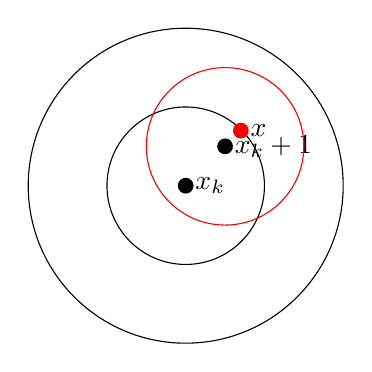
\begin{tikzpicture}
			\draw (0,0) circle(2);
			\fill (0,0) circle (.1);
			\node at (0,0) [right] {$x_k$};
			\draw (0,0) circle(1);
			\fill (0.5,0.5) circle (.1);
			\node at (0.5,0.5) [right] {$x_k+1$};
			\draw[red] (0.5,0.5) circle(1);
			\fill[red](0.7,0.7) circle (.1);
			\node at (0.7,0.7) [right] {$x$};
		\end{tikzpicture}
	\end{note}
	\begin{theorem}[$\textbf{纲定理}$]
		任何完备的度量空间均为第二类型的集。
	\end{theorem}
	\begin{proof}
		假设结论不对,则存在完备距离空间$\mathscr{X}$,使得$\mathscr{X}$为第一类型的集,于是有\begin{equation*}
			\mathscr{X}=\bigcup_{n=1}^{\infty}F_n
		\end{equation*}
		其中$F_n, (n=1,2,\cdots)$均为稀疏集.\\
		$\forall$闭球$\overline{S}(x_0,r_0)\subset \mathscr{X}$.由$F_1$是稀疏集,于是$\exists
		\overline{S}(x_1,r_1)\subset \overline{S}(s_0,r_0),s.t. $\begin{equation*}
			\overline{S}(x_1,r_1)\cap F_1=\varnothing
		\end{equation*}
		这里不妨设$0<r_1<1$;\\
		由于$F_2$是稀疏集,所以同理,$\exists \overline{S}(x_2,r_2)\subset
		\overline{S}(s_1,r_1),s.t. $\begin{equation*}
			\overline{S}(x_2,r_2)\cap F_2=\varnothing
		\end{equation*}
		这里不妨设$0<r_2<\frac{1}{2}$\\
		依此类推,我们找到一列闭球套:\begin{equation*}
			\overline{S}(x_1,r_1)\supset \overline{S}(x_2,r_2)\supset \cdots
			\overline{S}(x_n,r_n)\supset\cdots
		\end{equation*}
		其中$r_n$满足:$1<r_n<\frac{1}{n}$,因此$\{r_n\}\to
		0$,而且我们知道$\overline{S}(x_n,r_n)$不含$F_1,F_2,\cdots,F_n$中的点,$n=1,2,\cdots$ \\
		另一方面,由于$\mathscr{X}$是完备空间,则$\exists y_0\in
		\bigcap_{n=1}^{\infty}\overline{S}(x_n,r_n)$,故$y_0\in\mathscr{X}.$\\
		但是根据上述假设得出的结果,显然$y_0\notin F_n(n=1,2,\cdots).$从而$y_0\notin \mathscr{X}.$矛盾!
	\end{proof}
	\section{准紧集及紧集}
	\begin{definition}[$\textbf{有界}$]
		距离空间$\mathscr{X}$中的子集A称为$\textbf{有界}$,如果A包含在$\mathscr{X}$中的某个开球或闭球内。
	\end{definition}
	\begin{definition}[$\textbf{准紧集、紧集}$]
		\begin{description}
			\item[$\textbf{准紧集}$] 	设$A\subset
			\mathscr{X}$,如果A中的每个点列都含有子列收敛于$\mathscr{X}$中的某一点,则称A为$\textbf{准紧集}.$
			\item[$\textbf{紧集}$] 如果A中的每个点列都含有子列收敛于A中的某一点,则称A为$\textbf{紧集}.$
			\item[$\textbf{近距离空间}$] 如果空间$\mathscr{X}$自身是紧集.
		\end{description}
	\end{definition}
	\begin{note}
		\begin{itemize}
			\item $L^2[-\pi,\pi]$中的三角函数系$\begin{Bmatrix}
				\frac{1}{\sqrt{2\pi}},\frac{1}{\sqrt{\pi}}\cos t,\frac{1}{\sqrt{\pi}} \sin
				t,\cdots,\frac{1}{\sqrt{\pi}}\cos nt,\frac{1}{\sqrt{\pi}}\sin nt,\cdots
			\end{Bmatrix}$是有界的,但任意两个元素间的距离都大于1,于是不可能存在收敛的子列,因此不是准紧集
			\item $C[a,b]$上,考察点列\begin{equation*}
				x_n(t)=\left\{\begin{matrix}
					0 &\quad t\geqslant \frac{1}{n} \\ 
					1-nt&\quad t\leqslant  \frac{1}{n}
				\end{matrix}\right.
				\qquad	(n=1,2,\cdots)
			\end{equation*}
			显然,$\{x_n\}\subset B(\theta,1)$,其中$\theta$表示恒为0的函数,但是$\{x_n\}$不含有收敛子列。
		\end{itemize}
	\end{note}
	\begin{note}
		下列事实成立:\begin{enumerate}
			\item 任何有限集都是紧集
			\item 任何准紧集的子集都是准紧集
			\item 任何紧集的闭子集都是紧集
		\end{enumerate}
	\end{note}
	\begin{definition}[$\epsilon-\textbf{网}$]
		设$M,N\subset (\mathscr{X},\rho),\epsilon >0$,\\
		若对于$\forall x\in M,\exists y \in N,s.t.\quad
		d(x,y)<\epsilon$,则称N是M的一个$\epsilon\textbf{网}$;\\
		若N是一个有穷集,则称N为M的一个$\textbf{有穷}\epsilon\textbf{网}.$
	\end{definition}
	\begin{definition}[$\textbf{全有界集}$]
		若对于$\forall \epsilon>0$,A总存在着有限的$\epsilon-$网,则称A是$\textbf{全有界集}.$
	\end{definition}
	\begin{note}
		全有界集有以下的性质:
		\begin{enumerate}
			\item 任何有限集合都是全有界的
			\item 全有界集的子集也是全有界的
			\item 设A为全有界集,则对$\forall \epsilon>0$,总可以取A的一个有限子集作为A的$\epsilon-$网
			\\
			证明不妨设A的$\epsilon/2-$网中的元素全都不属于A,那么找以这些点为球心,半径为$\epsilon
			/2$的球与A的交集,从这些有限个集合中选一个组成集合就证明了。
		\end{enumerate}
	\end{note}
	\begin{theorem}
		全有界$\Rightarrow$有界,可分
	\end{theorem}
	\begin{proof}
		设$(\mathscr{X},\rho)$是一个度量空间,并设$A\subset \mathscr{X}$是全有界的。\\
		先证明有界:\\
		设$B=\{x_1,x_2,\cdots,x_{n_0}\} $是A的一个1-网,因此$\forall x\in A,\exists x_k\in
		B,s.t.$\begin{equation*}
			\rho(x,x_k)<1
		\end{equation*}
		故
		\begin{equation*}
			\rho(x,x_{n_0})\leqslant \rho(x,x_k)+\rho(x_k,x_{n_0})<1+\underset{1\leqslant k
				\leqslant n_0}{max}\rho(x_k,x_{n_0})=1+K
		\end{equation*}
		其中,$\underset{1\leqslant k \leqslant n_0}{max}\rho(x_k,x_{n_0})$是有限数,故A有界。\\
		下证可分:\\
		设$B_n$是A的有限$\frac{1}{n}-$网,且$B_n\subset A$,它们的并集\begin{equation*}
			B=\bigcup_{n=1}^{\infty}B_n
		\end{equation*}
		可列.\\
		$\forall x\in A ,\exists x_n \in B_n,s.t. \rho(x,x_n)<\frac{1}{n}$.\\
		故点列$\{x_n\}\to x$,从而可知,B在A中稠密,故A可分。
	\end{proof}
	\begin{theorem}
		设$(\mathscr{X},\rho)$为一度量空间,$A\subset \mathscr{X}$,则A准紧集$\Rightarrow $A全有界\\
		若$(\mathscr{X},\rho)$完备,则A准紧集$\Leftarrow $A全有界.
	\end{theorem}
	\begin{proof}
		$\Rightarrow \quad$否则,$\exists \epsilon_0>0,s.t. A$没有有限的$\epsilon$网 \\
		构造$\{x_n\}$\\
		任取$x_1\in A$\\
		又取$x_2\in A,s.t. \quad \rho(x_2,x_1)\geqslant
		\epsilon_0$(如果不能取那么$\{x_1\}$就是A的一个$\epsilon_0$网)\\
		$\cdots$\\
		取$x_n\in A,s.t. \quad \rho(x_n,x_1)\geqslant \epsilon_0$\\
		则$\{x_n\}$没有收敛的子列,与A是准紧集矛盾。\\
		$\Leftarrow \quad$任取A中点列$\{x_n\}$\\
		若$\{x_n\}$中只有有限个互不相同的元素,则显然$\{x_n\}$中含有收敛子列,\\
		若$\{x_n\}$中由无限多个互不相同的元素,用$B_0$记这些元素构成的集合,\\
		$A\subset \mathscr{X}$是全有界集,则$B_0$全有界,\\
		$B_0$中存在有限个元素,以它们为球心,$\frac{1}{2}$为半径作开球$\supset B_0$,\\
		于是至少存在一个开球包含$B_0$中无限多个元素,\\
		又$\exists B_2\subset B_1,s.t. B_2$中含有$B_1$中无限多个元素,且直径$\leqslant \frac{1}{2}$,\\
		依此类推\begin{equation*}
			B_1\supset B_2 \supset \cdots\supset B_k\supset \cdots
		\end{equation*}
		其中$B_n$的直径$\leqslant \frac{1}{2^{n-1}}$,\\
		取$x_{n_1}\in \{x_n\}\bigcap B_1$,\\
		$x_{n_2}\in \{x_n\}\bigcap B_2$,且$n_2>n_1$,\\
		$\cdots$\\
		$\{x_{n_k}\}$是基本列,由于$\mathscr{X}$完备,故在$\mathscr{X}$中收敛,从而A准紧。
	\end{proof}
	\begin{theorem}
		设$\{K_n\}$为距离空间$\mathscr{X}$中的一非空紧集序列,满足\begin{equation*}
			K_1\supset K_2 \supset \cdots \supset K_n \supset \cdots
		\end{equation*}
		则它们的交$\bigcap_{n=1}^{\infty}K_n$非空。
	\end{theorem}
	\begin{proof}
		
		在每个$K_n$中任取一点$x_n$,构成点列$\{x_n\}$.因为$K_1$是紧集,所以存在子列$\{x_{n_k}\}$,在$K_1$中收敛到$x_0$,由于$K_n$是闭集,所以$x_0\in
		K_n\quad(n=1,2,\cdots)$,即$x_0\in \bigcap_{n=1}^{\infty}K_n$
	\end{proof}
	\begin{theorem}
		设$\mathscr{X}$是距离空间,A$\subset \mathscr{X}$,\\
		A具有有限覆盖定理(A可以是开集)$\Leftrightarrow $A是紧集$\Leftrightarrow
		$(这里A必须是闭紧集)A中每个具有有限交性质的闭子集族(任一有限子族具有非空的交)$\{F_c\}_{c\in J}$有非空的交。
	\end{theorem}
	\begin{proof}
		内容...
	\end{proof}
	\section{某些具体空间中集合准紧性的判别法}
	\begin{theorem}
		集合A$\subset C[a,b]$准紧
		$\Leftrightarrow$\\
		\begin{description}
			\item[1)] A有界,即存在常数K,是对一切$x\in A$,有$\left | x(t)\right |\leqslant K$
			\item[2)] A等度连续,即$\forall \epsilon >0$,$\exists \delta >0,s.t. $对$\forall
			t',t'' \in A$,只要$\left |t'-t'' \right |<\delta$,就有\begin{equation*}
				\left |x(t')-x(t'') \right |<\epsilon ,\forall x\in A.
			\end{equation*}
		\end{description}
	\end{theorem}
	\begin{proof}
		$\Rightarrow $由于A是准紧集,所以A是全有界的,于是A有界;\\
		再证:A等度连续。\\
		由于A是准紧集,故$\exists A$的有限$\frac{\epsilon}{3}$-网$\{x_j\}_{j=1}^{n_0}$,对于$\forall
		x\in A$,有$x_{j_0},s.t. $\begin{equation*}
			\rho(x,x_{j_0})<\frac{\epsilon}{3}
		\end{equation*}
		\begin{equation*}
			\left | x(t')-x(t'')\right |\leqslant \left | x(t')-x_{j_0}(t')\right |+\left
			| x_{j_0}(t')-x_{j_0}(t'')\right |+\left | x_{j_0}(t'')-x(t'')\right |<\epsilon
		\end{equation*}
		故等度连续证毕。\\
		$\Leftarrow$ 设A有界且等度连续\\
		根据等度连续的定义,对于$\forall \epsilon >0,\exists \delta ,s.t.\forall t',t''\in
		[a,b]$,只要$\left | t'-t''\right |<\delta$,就有\begin{equation*}
			\left | x(t')-x(t'')\right |<\epsilon,\quad \forall x \in A
		\end{equation*}
		将$[a,b]$n等分,区间端点为$a=t_0<t_1<\cdots<t_n=b$,使得每个区间长度$<\delta$.\\
		作点集:\begin{equation*}
			\hat{A}=\{x(t_0),x(t_1),\cdots,x(t_n):x\in A\}\subset \mathbf{R}^{n+1}
		\end{equation*}
		A有界$\Rightarrow \hat{A}$有界$\Rightarrow \hat{A}$是准紧集$\overset{\mathbb{R}^n
			\textbf{是完备集} }{\Rightarrow }$A全有界.\\
		从而$\forall \epsilon >0,\exists \{x_j(t)\}_{j=1}^m\subset
		A$,$s.t$\begin{equation*}
			\{(x_j(t_0),\cdots,x_j(t_n))\}_{j=1}^m
		\end{equation*}
		为$\hat{A}$的$\epsilon-$网($\mathbb{R}^n$是完备集,所以A全有界。)\\
		$\forall t \in[a,b]$,有\begin{equation*}
			\left | x(t)-x_{j_0}(t)\right |\leqslant \left | x(t)-x(t_j)\right |+\left |
			x(t_j)-x_{j_0}(t_j)\right |+\left | x_{j_0}(t_j)-x_{j_0}(t)\right | <\epsilon
		\end{equation*}右边第一项和第三项是等度连续,第二项是因为$\epsilon$网。
	\end{proof}
	\begin{definition}[$\textbf{映射}$]
		设$\mathscr{X},\mathscr{Y}$都是距离空间,距离分别为$\rho,\rho_1.$如果对每一个$x\in
		\mathscr{X}$,按照某个规律必有$\mathscr{Y}$中的y与之对应,则称这个对应是一个$\textbf{映射}$.
	\end{definition}
	\begin{note}
		单射,满射,定义域,值域,原像,像定义省略
	\end{note}
	\begin{definition}
		对于$\forall \epsilon >0,\exists \delta
		>0,s.t.$当$\rho(x,x_0)<\delta$时,有$\rho_1(Tx,Tx_0)<\epsilon$,则称映射T在点$x_0$处$\textbf{连续}$。
	\end{definition}
	\begin{note}
		$T:\mathscr{X}\to\mathscr{Y}$连续$\Leftrightarrow$T在$\mathscr{X}$上每一点都连续.
	\end{note}
	\begin{theorem}
		以下等价:\begin{enumerate}
			\item T:$\mathscr{X}\to\mathscr{Y}$连续
			\item $\mathscr{Y}$中的任一开集$G$,$T^{-1}(G)$是X中的开集
			\item $\mathscr{Y}$中的任一闭集$G$,$T^{-1}(G)$是X中的闭集
		\end{enumerate}
	\end{theorem}
	\begin{definition}
		\begin{enumerate}
			\item $\textbf{同胚映射}$:$T,T^{-1}$都连续.
			\item $\textbf{等距映射}$:$\forall x,y\in \mathscr{X}$,有$\rho_1(Tx,Ty)=\rho(x,y)$
			\item $\textbf{等价度量同构}$:$\exists c\geqslant 1,s.t. c^{-1}\rho(x,y)\leqslant
			\rho(Tx,Ty)\leqslant c\rho(x,y),\forall x,y\in \mathscr{Z}.$
		\end{enumerate}
	\end{definition}
	\begin{note}
		性质:
		\begin{enumerate}
			
			\item 设$A$是$\mathscr{X}$中的紧集,$\exists f:A\to \mathscr{R}$连续,\\
			$\Rightarrow \exists x_0\in A,s.t. f(x_0)=\underset{x\in A}{sup}f(x)$\\
			因为$\mathscr{R}$是稠密集,所以有$\{x_n\}\in A,s.t. f(x_n)\to \underset{x\in
				A}{sup}f(x)$\\
			又因为A是紧集,所以$\exists \{x_{n_k}\}\to x_0,s.t.f(x_{n_k})\to f(x_0).$
			\item 一致连续与一维欧氏空间上的定义大同小异。
		\end{enumerate}
	\end{note}
	\section{不动点定理}
	\begin{definition}[$\textbf{不动点}$]
		对于映射T,$\exists x,s.t.Tx=x$,x称为映射T的不动点.
	\end{definition}
	\begin{definition}
		\begin{enumerate}
			\item $\textbf{压缩}$:若$\exists \alpha \in(0,1),s.t.$\begin{equation*}
				\rho(Tx,Ty)\leqslant\alpha\rho(x,y),\quad \forall x,y\in \mathscr{X}
			\end{equation*}
			\item $\textbf{非扩张的压缩}$
		\end{enumerate}
	\end{definition}
	\begin{theorem}[$\textbf{不动点定理}$]
		设$\mathscr{X}$完备,距离为$\rho$.T:$\mathscr{X}\to\mathscr{X}$,且对于$\forall x,y\in
		\mathscr{X}$,不等式\begin{equation*}
			\rho(Tx,Ty)\leqslant \theta\rho(x,y)
		\end{equation*}
		成立,其中$0\leqslant \theta<1$,那么T在$\mathscr{X}$中存在唯一的不动点.
	\end{theorem}
	\begin{proof}
		任取$x_0 \in \mathscr{X}$,令\begin{equation*}
			x_n=Tx_{n-1} \quad n=1,2,\cdots
		\end{equation*}
		\begin{description}
			\item[step1] 先证明$\{x_n\}$是一个基本点列:\\
			利用归纳法可证得:\begin{equation*}
				\rho(x_n,x_{n+1})=\rho(Tx_{n-1},Tx_n)\leqslant \theta \rho(x_{n-1},x_n)
				\leqslant \cdots \leqslant \theta ^n\rho(x_0,Tx_0)
			\end{equation*}
			于是有\begin{align*}
				\rho(x_n,x_{n+p})&\leqslant \rho(x_n,x_{n+1})+\cdots +\rho(x_{n+p-1},x_{n+p})\\
				&\leqslant (\theta^n+\cdots+\theta^{n+p-1})\rho(x_0,Tx_0)\\
				&\leqslant \frac{\theta^n(1-\theta^p)}{1-\theta}\rho(x_0,Tx_0)\\
				&\leqslant \frac{\theta^n}{1-\theta}\to 0
			\end{align*}
			所以$\{x_n\}$是$\mathscr{X}$中的基本点列\\
			又因为$\mathscr{X}$是完备的,故$\{x_n\}\to x\in \mathscr{X}$\\
			又$\rho(Tx,Ty)\leqslant \theta \rho(x,y)\Rightarrow $T是连续映射.\\
			从而\begin{equation*}
				x\leftarrow x_{n+1}=Tx_n\to Tx
			\end{equation*}
			即$x=TX$.
			\item[step2] 再证不动点的唯一性.\\
			设另存在$y\in \mathscr{X},s.t. y=Ty$,则\begin{equation*}
				\rho(x,y)=\rho(Tx,Ty) \leqslant \theta\rho(x,y)\Rightarrow x=y
			\end{equation*}
		\end{description}
	\end{proof}
	\begin{problem}
		微分方程解的存在性与唯一性:微分方程\begin{equation*}
			\left\{\begin{matrix}
				\frac{dy}{dx}=p(x,y)\\ 
				y(x_0)=y_0
			\end{matrix}\right.
		\end{equation*}
		其中$f\in C(\mathbb{R}^2)$\\
		设$y$满足Lipschitz条件,即$\exists K>0,s.t.$\begin{equation*}
			\left | f(x,y)-f(x,y')\right | \leqslant K\left | y-y'\right |
		\end{equation*}
	\end{problem}
	\begin{solution}
		\begin{align*}
			y(x)-y_0&=\int_{x_0}^{x}\frac{dy}{dx}dx\\
			&=\int_{x_0}^{x}f(x,y(x))dx\\
			&=\int_{x_0}^{x}f(t,y(t))dt
		\end{align*}
		(可以看出这个解的结构但无法说明解的存在性与唯一性,但是积分不一定收敛)\\
		取$\delta >0,s.t. k\delta <1$,在$C[x_0-\delta,x_0+\delta]$上定义T:\begin{equation*}
			(Ty)(x)=y_0+\int_{x_0}^{x}f(t,y(t))dt
		\end{equation*}
	则\begin{align*}
		\rho(Ty_1,Ty_2)&=\underset{\left | x-x_0\right |\leqslant \delta}{max}\left | \int_{x_0}^{x}[f(t,y_1(t))-f(t,y_2(t))]dt\right | \\
		&\underset{\leqslant}{Lipschitz} \underset{\left | x-x_0\right |\leqslant \delta}{max}\int_{x_0}^{x}K\left | y_1(t)-y_2(t)\right |dt\\
		&\leqslant K\delta \underset{\left | t-x_0\right |\leqslant \delta}{max}\left | y_1(t)-y_2(t)\right |\\
		&=K\delta \rho(y_1,y_2)
	\end{align*}
$K\delta <1$,故由不动点定理:$y=y_0(x)$是微分方程通过点$(x_),y_0)$的唯一积分曲线,再令$y(x_0\pm \delta)=y_0(x_0\pm \delta)$,延拓,可得在整个实数轴上的解.
	\end{solution}
\begin{problem}
	积分方程解的存在性与唯一性:积分方程\begin{equation*}
		x(t)=f(t)+\lambda \int_{a}^{b}K(t,s)x(s)ds
	\end{equation*}
	$f\in L^2[a,b],K(t,s)\in [a,b]\times [a,b]$,且$\int_{a}^{b}\int_{a}^{b}\left | K(t,s)\right |^2dtds<\infty$\\
	则当$\lambda$充分小时,$\exists !x\in L^2[a,b],s.t.$满足上述方程.
\end{problem}
\begin{solution}
令\begin{equation*}
	(Tx)(t)=f(t)+\lambda \int_{a}^{b}K(t,s)x(s)ds
\end{equation*}
则\begin{align*}
	\rho(Tx,Ty)&\leqslant \left | \lambda\right |(\int_{a}^{b}\left | \int_{a}^{b}K(t,s)(x(s)-y(s))ds\right |^2dt)^{1/2}\\
	&\leqslant \left | \lambda\right |\left \{\int_{a}^{b}\left [ \int_{a}^{b}\left | K(t,s)\right |^2ds\int_{a}^{b}\left | x(s)-y(s)\right |^2ds\right ]dt\right \}^{1/2}\\
	&=\left | \lambda\right |\left ( \int_{a}^{b}\int_{a}^{b}\left | K(t,s)\right |^2dsdt\right )^{1/2}\cdot \left ( \int_{a}^{b}\int_{a}^{b}\left | x(s)-y(s)\right |^2dsdt\right )^{1/2} \\
	&=I_1\cdot I_2
\end{align*}
令$\lambda$充分小,$s.t. I_1<1$,则有\begin{equation*}
	\rho(Tx,Ty)\leqslant I_1 \cdot \rho(x,y)
\end{equation*}
故T为压缩映射.\\
从而方程存在唯一的解.
\end{solution}
\begin{problem}
	V.Volterra积分方程:设$K(t,s)\in C[a,b]\times[a,t]$(三角形区域),则Volterra方程\begin{equation*}
		x(t)=\lambda \int_{a}^{t}K(t,s)x(s)ds+f(t)
	\end{equation*}
对$\forall f\in C[a,b],\lambda,\exists !x_0\in C[a,b]$是方程的解.
\end{problem}
\chapter{巴拿赫空间与希尔伯特空间}
\section{赋范空间及内积空间}
\begin{definition}[$\textbf{线性空间}$]
	E非空,K实(复)数域,则称E是实(复)线性空间,若满足:\begin{itemize}
		\item 加法:$E \times E\to E$\begin{description}
			\item[1)] 结合律
			\item[2)] 交换律
			\item[3)] 零元素:$\exists !\theta \in E,s.t. x+\theta =x,\forall x \in E$
			\item[4)] 逆元素:$\forall x\in E,\exists -x\in E,s.t. x+(-x)=\theta $
		\end{description}
	\item 乘法:$K\cdot E\to E$\begin{description}
		\item[1)] 结合律:$\alpha ,\beta \in K,x\in E$,满足$\alpha (\beta x)=(\alpha \beta )x=(\beta \alpha )x$
	\item[2)] 单位元:1$\cdot x$=x
	\end{description}
\item 相容性:分配律\begin{description}
	\item[1)] $(\alpha +\beta)x=\alpha x+\beta x$
	\item[2)] $\alpha (x+y)=\alpha x+\beta y$
\end{description}
	\end{itemize}
\end{definition}
\begin{note}
	推证:\begin{description}
		\item[1)] (-1)x=-x
		\item[2)] $\alpha x=\theta \Leftrightarrow \alpha =0$或$x=\theta$
		\item[3)] $0\cdot x=\theta,\alpha \cdot \theta =\theta$
	\end{description}
\end{note}
\begin{note}
	线性相关$\Leftrightarrow $维数$\Leftrightarrow $无限维(即有任意个元素的无关组)
\end{note}
\begin{definition}
	\begin{itemize}
		\item $\textbf{子空间}$ 
		$E_0\subset E,\forall \alpha \in K,\forall x,y, \in E_0 \Leftrightarrow x+y\in E_0,\alpha x\in E_0$,容易验证:$E_0$是线性空间,称$E_0$是E的子空间.
		\item $\textbf{A的张成}$
	SpanA=$\left \{\sum_{j=1}^{m}\alpha _jx_j\mid \alpha_j\in K,x_j\in A\subset E,m\in \mathbb{N}\right \}$
	容易验证:SpanA是E的子空间.
\item $\textbf{线性同构}$
	$\mathscr{X}$与$\mathscr{Y}$为线性空间,称$\mathscr{X}$与$\mathscr{Y}$线性同构,若$\exists$ 线性双射:T:$\mathscr{X}\to \mathscr{Y}$,s.t.\begin{equation*}
		\left\{\begin{matrix}
			T(x+y)=Tx+Ty\\ 
			T(\alpha x)=\alpha Tx
		\end{matrix}\right.
	\end{equation*}

\item $\textbf{直和}$
	$L_j(j=1,\cdots,n)$均为$\mathscr{X}$的子空间,若对$\forall x \in L\overset{\triangle}{=}\underset{j=1}{\overset{n}{\oplus }}L_j$有唯一分解:\begin{equation*}
		x=\sum_{j=1}^{n}x_j,\quad x_j\in L_j
	\end{equation*}
则称L为$\{L_j\}_{j=1}^{n}$的直和.(显然L是一个线性空间)
		\end{itemize}
\end{definition}
\begin{note}
	例:$\mathbb{R}^n=\underset{j=1}{\overset{n}{\oplus }}\mathbb{\widetilde{R_j}}$\\
	其中$\mathbb{\widetilde{R_j}} \overset{\triangle}{=}\left \{(0,\cdots,x_j,0,\cdots,0)\mid x_j\in \mathbb{R}\right \}$与$\mathbb{R}$线性同构.
\end{note}
\begin{definition}[$\textbf{商空间}$]
	设$E$线性空间,$L\subset E$是E的子空间.
	\begin{itemize}
		\item 定义等价关系$(x\sim y)$:$x,y\in E,\quad x-y\in L$(满足自反性,对称性,传递性)
		\item 等价类:\begin{align*}
			\hat{x}=x+L\\
			\hat{x}=\hat{y}\Leftrightarrow x+L=y=L\Leftrightarrow x-y\in L\Leftrightarrow x\sim y
		\end{align*}
	\item 商空间:$\mathbb{Z}/_L=\mathbb{Z}/_{\sim L}\overset{\triangle}{=}\{${所有等价类}$\}$,线性结构如下定义:\begin{enumerate}
		\item 加法:$\hat{x}+\hat{y}\overset{\triangle }{=}\widehat{x+y}$
		\item 乘法:$\alpha \hat{x}\overset{\triangle }{=} \alpha x+L=\widehat{\alpha x}$
	\end{enumerate}
容易验证如此定义的结构是线性的.
	\end{itemize}
\end{definition}
\begin{note}
	例:$L^P(F)$是一个商空间(常常规定其中任一a.e.相等的函数为同一函数)\\
	令$\widetilde{L}=\left \{g:g\overset{a.e.}{\underset{on F}{=}}0\right \}$,则$L^P(F)=\{$p幂可积函数$\}/_{\widetilde{L}}$
\end{note}
\begin{definition}[$\textbf{赋范线性空间}$]:$\mathscr{X}+$线性结构$+$(度量)拓扑结构\\
	设$\mathscr{X}$为线性空间,定义范数:$\left \| \cdot \right \|:\mathscr{X}\to [0,\infty)$,满足\begin{description}
		\item[1)] $\left \| x\right \|\geqslant 0$,且$\left \| x\right \|= 0\Leftrightarrow x=\theta$
		\item[2)] $\left \| \alpha x\right \|=\left | \alpha\right |\left \| x\right \|$(距离空间中没有这个线性条件)
		\item[3)] $\left \| x+y\right \|\leqslant \left \| x\right \|+\left \| y\right \|$
	\end{description}
	则称$\mathscr{X}$是线赋范线性空间.
\end{definition}
\begin{note}
	性质:\begin{description}
		\item[1)] 赋范$\Rightarrow$度量
		\item[2)] 线性运算关于E中的收敛是连续的.
		\begin{itemize}
			\item $x_n\to x \Rightarrow \left \| x_n\right \|\to \left \| x\right \|$\\
			$x_n\to x \Leftrightarrow \left \| x_n-x\right \|\to 0 \Rightarrow \begin{vmatrix}
				\left \| x_n\right \|-\left \| x\right \|
			\end{vmatrix}\leqslant \left \| x_n-x\right \|\to 0$\\
		即$\left \| x_n\right \|\to \left \| x\right \|$
		\item $x_n\to x,y_n\to y\Rightarrow x_n+y_n\to x+y$\\
		$\left \| x_n+y_n-x-y\right \|\leqslant \left \| x_n-x\right \|+\left \| y_n-y\right \|$
		\item $\alpha _n\to \alpha,x_n\to x \Rightarrow \alpha_n x_n\to \alpha x$\\
	$
			\left \| \alpha_nx_n-\alpha x\right \|=\left \| (\alpha_n-\alpha)x_n+\alpha(x_n-x)\right \|\\
			\leqslant \left | \alpha_n -\alpha\right |\left \| x_n\right \|+\left | \alpha\right |\left \| x_n-x\right \|\\
			\to 0
$
		\end{itemize}
	\end{description}
\end{note}
\begin{note}
	赋范空间例子\\ 
	\begin{itemize}
		\item $\mathbb{R}\quad (\left \| x\right \|=(\sum_{k=1}^{n}\left | \xi _k\right |^2)^{1/2})$
		\item $C[a,b]\quad (\left \| x\right \|=\underset{a\leqslant t\leqslant b}{max}\left | x(t)\right |)$
		\item $L^P(F)\quad (\left \| x\right \|=(\int _F\left | x(t)\right |^pdt)^{1/p})$
		\item $l^p(F) \quad (\left \| x\right \|=(\sum_{n=1}^{\infty}\left | \xi_n\right |^pdt)^{1/p}) \quad (x=\{\xi _1,\xi_2,\cdots, \xi_n\},\sum_{n=1}^{\infty}\left | \xi_n\right |^p<\infty)$
		\item $L^{\infty}(F)\quad (\left \| x\right \|=\underset{mF_0=0,F_0\subset F}{inf}\left[\underset{F\setminus F_0}{sup}\left | x(t)\right |]\right])$
(除零测集外有界,上确界的下确界)
	\end{itemize}
\end{note}
\begin{definition}[$\textbf{巴拿赫空间}$]
	完备的赋范空间
\end{definition}
\begin{definition}
	\begin{itemize}
		\item $\textbf{赋范空间的直和}\quad L_1,L_2,\cdots,L_n$是赋范空间,$E=L_1\oplus L_2\oplus \cdots \oplus L_n$,在E中定义范数:\begin{equation*}
			\left \| x\right \|\overset{\triangle }{=}\sum_{i=1}^{n}\left \| x_i\right \|
		\end{equation*} 
	容易验证$\left \| x\right \|$满足范数定义的全部条件,故E按范数$\left \| \cdot \right \|$是一个线性赋范空间.
	\item $\textbf{赋范空间的维数}\quad $ E是一个赋范空间,$\exists \{e_k\}_{k=1}^n \subset E,s.t.\forall x\in E,\exists !\{c_k\}_{k=1}^n$,满足\begin{equation*}
	   x=\sum_{k=1}^{n}c_ke_k
	\end{equation*}
则$\{e_k\}_{k=1}^n $是E的基,n是E的维数.
\item $\textbf{Schauder基}\quad $在上述基的基础上,E是一个无限维的巴拿赫空间(完备的赋范空间),满足\begin{equation*}
	x=\sum_{k=1}^{\infty}c_ke_k
\end{equation*}
且\begin{equation*}
	\left \| \sum_{k=1}^{n}c_ke_k-x\right \|\to 0 \quad (n\to \infty)
\end{equation*}
则$\{e_k\}_{k=1}^{\infty}$是Schauder基.
	\end{itemize}
\end{definition}
\begin{note}
	例:$E=l^p$是按$\left \| x\right \|=\left ( \sum_{j=1}^{\infty}\left | \xi_j\right |^p\right )^{1/p}$的赋范空间,则$\{e_j\}_{j=1}^{\infty}=\{(0,\cdots,0,\cdots)\}$是$l^p$的一组基.\\
	pf:即证:$\forall x\in l^p$,可唯一地被表示成\begin{equation*}
		x=\sum_{j=1}^{\infty}x_je_j
	\end{equation*}
其中,$x=(x_1,x_2,\cdots,x_j,\cdots)$
\begin{description}
	\item[step1] 先证:级数$\sum_{j=1}^{\infty}x_je_j$收敛\begin{align*}
		\left \| \sum_{j=1}^{m}x_je_j-\sum_{j=1}^{n}x_je_j\right \|_{l^p}&=\left \| \sum_{j=n+1}^{m}x_je_j\right \|_{l^p}\\
		&=\left \| (0,\cdots,x_{n+1},\cdots,x_m,\cdots)\right \|_{l^p}\\
		&=\left ( \sum_{j=n+1}^{m}\left | x_j\right |^p\right )^{1/p}\to 0(n,m\to\infty)
  	\end{align*}
  (因为$x\in l^2$,所以$\left \| x\right \|=\left ( \sum_{j=1}^{\infty}\left | x_j\right |^p\right )^{1/p}$收敛,所以上述证明合理.)
  \item[step2] 再证$\sum_{j=1}^{\infty}x_je_j\to x$\begin{align*}
  	\left \| x-\sum_{j=1}^{n}x_je_j\right \|&=\left \| (0,\cdots,0,x_{n+1},x_{n+2},\cdots)\right \|_{l^p}\\
  	&=\left ( \sum_{j=n+1}^{\infty}\left | x_j\right |^p\right )^{1/p}\to 0\quad (n\to \infty)p
  \end{align*}
\end{description}
\end{note}
\begin{definition}
	E,$E_1$是赋范空间,且E与$E_1$作为线性空间是同构(线性映射)的.\begin{itemize}
		\item $\textbf{等距同构:} T:E\to E_1$,满足$\left \| Tx-Ty\right \|_{E_1}=\left \| x-y\right \|_E$
		\item $\textbf{拓扑同构:} T:E\to E_1$,满足T是同胚映射($T,T^{-1}$均为连续映射)
	\end{itemize}
\end{definition}
\begin{note}
例子:证明	$\forall E_1,E_2$为实(复)n维赋范线性空间,则$E_1\cong E_2$\\
	pf:不妨设$E$是实赋范空间,且$\{e_j\}_{j=1}^n$是E的一组基,只需证$E\cong \mathbb{R}^n$\\
	Define:$T:\mathbb{R}^n \to E,\quad (x_1,x_2,\cdots,x_n)\mapsto x_1e_1+x_2e_2+\cdots +x_ne_n$\begin{description}
		\item[step1] 证明T是线性连续双射\begin{description}
			\item[1)] $\{e_j\}_{j=1}^n$线性无关$\Rightarrow $T是单射\\
			又$\forall y=y_1e_1+\cdots +y_ne_n\in E,\exists (y_1,\cdots,y_n)\in \mathbb{R}^n,s.t.$\begin{equation*}
				T\left((y_1,\cdots ,y_n)\right)=y
			\end{equation*}
		故T是满射.
		\item[2)] 容易验证T是同构映射(线性双射)
		\item[3)] 下证:T是连续映射.\\
		\begin{align*}
			\left \| T(x_1,x_2,\cdots ,x_n)\right \|
			&=\left \| \sum_{j=1}^{n}x_je_j\right \|\\
			&\leqslant \sum_{j=1}^{n}\left | x_j\right |\left \| e_j\right \|\\
			&\overset{cauchy}{\leqslant }\left ( \sum_{j=1}^{n}\left | x_j\right |^2\right )^{1/2}\left ( \sum_{j=1}^{n}\left \| e_j\right \|^2\right )^{1/2}
		\end{align*}
	$\Rightarrow $\begin{align*}
		&\left \| T(x_1,\cdots,x_n)-T(y_1,\cdots,y_n)\right \|\\
		& \leqslant \left ( \sum_{j=1}^{n}\left \| e_j\right \|^2\right )^{1/2}\cdot \left [ \left ( \sum_{j=1}^{n}\left | x_j\right |^2\right )^{1/2}-\left ( \sum_{j=1}^{n}\left | y_j\right |^2\right )^{1/2}\right ]\\
		&\overset{Minkovski}{\leqslant }\left ( \sum_{j=1}^{n}\left \| e_j\right \|^2\right )^{1/2}\cdot \left ( \sum_{j=1}^{n}\left | x_j-y_j\right |^2\right )^{1/2}\\
		&=\left ( \sum_{j=1}^{n}\left \| e_j\right \|^2\right )^{1/2}\cdot \left \| (x_1,\cdots,x_n)-(y_1,\cdots ,y_n)\right \|
	\end{align*}
故T是连续双射.
		\end{description}
	\item[step2] 证明:$T^{-1}$连续.\\
	 对$\forall x=\sum_{j=1}^{n}x_je_j\in E$,有\begin{equation*}
	 	T^{-1}x=(x_1,x_2,\cdots,x_n)
	 \end{equation*}
 \begin{equation*}
 	\left \| T^{-1}(\frac{x}{\left \| T^{-1}x\right \|_{\mathbb{R}^n}})\right \|_{\mathbb{R}^n}\overset{\textbf{线性}}{=}\left \| \frac{1}{\left \| T^{-1}x \right \|_{\mathbb{R}^n}}T^{-1}x \right \|_{\mathbb{R}^n}
 \end{equation*}
故$T^{-1}(\frac{x}{\left \| T^{-1}x\right \|_{\mathbb{R}^n}})$位于$\mathbb{R}^n$中的单位球面上.\\
令\begin{equation*}
	x'=\frac{x}{\left \| T^{-1}x\right \|_{\mathbb{R}^n}}=\sum_{j=1}^{n}x_j'e_j
\end{equation*}
因为$\left \| x'\right \|_E$是一个关于$x_1',\cdots,x_n'$的连续函数,而单位球面在$\mathbb{R}^n$中是一个紧集。同时$\left \| x'\right \|_E>0$,从而$\left \| x'\right \|_E$在单位球面上由正的下确界,记为m.(上面有关于紧集的一些结论.)\\
从而有\begin{align*}
		\left \| x'\right \|_E \geqslant m & \Rightarrow \left \| x\right \|_E=\left \| T^{-1}x\right \|_{\mathbb{R}^n}\left \| x'\right \|_E\geqslant \left \| T^{-1}x\right \|m\\
	& \Rightarrow \left \| T^{-1}x\right \|_{\mathbb{R}^n}\leqslant \frac{1}{m}\left \| x\right \|_E\\
	& \Rightarrow \left \| T^{-1}x-T^{-1}y\right \|_{\mathbb{R}^n}\overset{\textbf{线性}}{=}\left \| T^{-1}(x-y)\right \|\leqslant \frac{1}{m}\left \| x-y\right \|
\end{align*}
故$T^{-1}$为连续线性映射.
	\end{description}
\end{note}
\begin{note}
$\mathscr{X}$是赋范线性空间,\begin{itemize}
	\item dim $\mathscr{X}=n,\Rightarrow \mathscr{X}$是巴拿赫空间;
	\item dim $\mathscr{X}=\infty,E\subset \mathscr{X}$,E是有限维子空间$\Rightarrow E$是$\mathscr{X}$的闭子空间.
\end{itemize}
\end{note}
\begin{definition}[$\textbf{内积空间}$]
$\mathscr{X}$是数域上的线性空间,$\forall x,y,z\in \mathscr{X}$,$\mathscr{X}$为内积空间,若\begin{description}
	\item[1)] $(\alpha x,y)=\alpha(x,y)$
	\item[2)] (x+y,z)=(x,z)+(y,z)
	\item[3)] \begin{itemize}
		\item k为实数域,(x,y)=(y,x)
		\item k为复数域,(x,y)=$\overline{(y,x)}$
	\end{itemize}
\item[4)] (x,x)$\geqslant 0$,且$(x,x)=0 \Leftrightarrow x=\theta$
\end{description}
\end{definition}
\begin{note}
性质:\begin{description}
	\item[1)] k实:$(x,y)$关于x,y线性;\\
	k复:$(x,\alpha_1y_1+\alpha_2y_2)=\overline{\alpha_1}(x,y_1)+\overline{\alpha_2}(x,y_2)$
	\item[2)] $\mathscr{X}$内积空间+范数定义:$\left \| x\right \|=\sqrt{(x,x)} \Rightarrow \mathscr{X}$赋范空间
	\begin{proof}
	\begin{description}
		\item[step1] schwarz不等式:\begin{equation*}
			\left | (x,y)\right |\leqslant \left \| x\right \|\cdot \left \| y\right \|
		\end{equation*}
	\begin{equation*}
		(x+\lambda y,x+\lambda y)=(x,x)+\overline{\lambda }(x,y)+\lambda(y,x)+\lambda \overline{\lambda}(y,y)\geqslant 0
	\end{equation*}
令\begin{equation*}
	\lambda =-\frac{(x,y)}{(y,y)}
\end{equation*}
则有\begin{equation*}
	(x,x)-2\frac{(x,y)\cdot (y,x)}{(y,y)}+\frac{(x,y)\cdot (y,x)}{(y,y)^2}(y,y)\geqslant 0
\end{equation*}
即\begin{equation*}
	\left | (x,y)\right |^2=(x,y)\overline{(x,y)}\leqslant (x,x)\cdot (y,y)=(\left \| x\right \|\left \| y\right \|)^2
\end{equation*}
\item[step2]  再证三角不等式\begin{equation*}
	\left \| x+y\right \|\leqslant \left \| x\right \|+\left \| y\right \|
\end{equation*}
\begin{align*}
	\left \| x+y\right \|^2&=\left | (x+y,x+y)\right |\\
	&=\left | (x+y,x)+(x+y,y)\right |\\
	&=\leqslant \left | (x+y,x)\right |+\left | (x+y,y)\right |\\
	&\leqslant \left \| x+y\right \|\cdot \left \| x\right \|+\left \| x+y\right \|\cdot \left \| y\right \|
\end{align*}
从而$\left \| x+y\right \|\leqslant \left \| x\right \|+\left \| y\right \|$
	\end{description}
又有$\left \| x\right \|\geqslant 0$且$\left \| x\right \|=0\Leftrightarrow x=\theta$,以及$\left \| \alpha x\right \|=\left | \alpha\right |\left \| x\right \|$可知按此定义范数内积空间可以构成赋范空间.
	\end{proof}
\item[3)] 相容性(拓扑与几何)\\
(x,y)是关于x与y的连续函数.\\
$\{x_n\},\{y_n\}\subset \mathscr{X}$,且\begin{align*}
	\left \| x_n-x\right \|\rightarrow 0,\left \| y_n-y\right \|\rightarrow 0 &\Rightarrow\\
	& \left | (x_n,y_n)-(x,y)\right |=\left | (x_n,y_n)-(x,y_n)+(x,y_n)-(x,y)\right|\\
    &	\leqslant \left \| x_n-x\right \|\left \| y_n\right \|+\left \| x\right \|\left \| y_n-y\right \|\rightarrow 0(n\to \infty)
\end{align*}
\item[4)] 由范数表示内积\begin{itemize}
	\item k是实数域 $(x,y)=\frac{1}{4}(\left \| x+y\right \|^2-\left \| x-y\right \|^2)$
	\item k是复数域$(x,y)=\frac{1}{4}\left( \left \| x+y\right \|^2-\left \| x-y\right \|^2+i(\left \| x+iy\right \|^2-\left \| x-iy\right \|^2) \right)$
\end{itemize}
\end{description}
\end{note}
\begin{definition}[$\textbf{希尔伯特空间}$]
	内积$\overset{\textbf{定义范数}}{\rightarrow }$内积空间+赋范空间$\left\{\begin{matrix}
		\overset{\textbf{完备}}{\rightarrow }\textbf{希尔伯特空间}\\ 
		\overset{\textbf{不完备}}{\rightarrow }\textbf{准希尔伯特空间}
	\end{matrix}\right. $
\end{definition}
\begin{note}
例子:\begin{itemize}
	\item 酉空间$\mathbb{C}^n\quad \left\{\begin{matrix}
		\textbf{内积}&(x,y)=\sum_{k=1}^{n}x_k\overline{y_k}\\
		\textbf{范数}&\left \| x\right \|=\sqrt{(x,x)}=\left ( \sum_{k=1}^{n}x_k\overline{x_k}\right )^{1/2}
	\end{matrix}\right.$
\item 空间$l^2 \quad \left\{\begin{matrix}
	\textbf{内积} (x,y)=\sum_{k=1}^{n}x_k\overline{y_k}  \\
	(\textbf{合理性:}\sum_{k=1}^{\infty}\left |x_k\overline{y_k} \right |\leqslant (\sum_{k=1}^{\infty}\left | x_k\right |^2)^{1/2}\cdot (\sum_{k=1}^{\infty}\left | \overline{y_k}\right |^2)^{1/2}  \textbf{于是}\sum_{k=1}^{\infty}x_k\overline{y_k}\textbf{收敛}) \\
	\textbf{范数} \left \| x\right \|=\sqrt{(x,x)}=\left ( \sum_{k=1}^{n}x_k\overline{x_k}\right )^{1/2} 
\end{matrix}\right.$
\item $L^2(F) \left\{\begin{matrix}
	\textbf{内积}(x,y)=\int _Fx(t)\overline{y(t)}dt\\ 
	\textbf{范数}\left \| x\right \|=\left ( \int _Fx(t)\overline{x(t)}dt\right )^{1/2}
\end{matrix}\right.$
\end{itemize}
\end{note}
\begin{note}
\begin{itemize}
	\item 用内积定义范数:$\left \| x\right \|=\sqrt{(x,x)}$
	\item 用范数定义内积:(x,y)=$\frac{1}{4}\left [ \left \| x+y\right \|^2-\left \| x-y\right \|^2+i(\left \| x+iy\right \|^2-\left \| x-iy\right \|^2)\right ]$
\end{itemize}
\end{note}
\begin{theorem}
\begin{equation*}
	\textbf{内积空间定义范数}\underset{(x,y)=\frac{1}{4}\left [ \left \| x+y\right \|^2-\left \| x-y\right \|^2+i(\left \| x+iy\right \|^2-\left \| x-iy\right \|^2)\right ]\textbf{+什么条件?}}{\overset{\left \| x\right \|=\sqrt{(x,x)}}{\rightleftharpoons }}\textbf{赋范空间}
\end{equation*}
\\
这个条件是\textbf{平行四边形公式}:$\left \| x+y\right \|^2+\left \| x-y\right \|^2=2\left \| x\right \|^2+2\left \| y\right \|^2$,容易验证,在这个条件下,以上按范数定义的内积满足形成内积的四个条件
\end{theorem}
\begin{note}例子:\\
$\mathbb{C}[a,b]$中,$\left \| x\right \|=\underset{t\in [a,b]}{max}\left | x(t)\right |$,但是不满足平行四边形公式\begin{equation*}\left \| x+y\right \|^2+\left \| x-y\right \|^2=2\left \| x\right \|^2+2\left \| y\right \|^2
\end{equation*}
所以无法按范数定义内积.
\end{note}
\section{希尔伯特空间(完备的内积+赋范空间)的正交系}
\begin{definition}[$\textbf{正交}$]
$\mathscr{X}$是内积空间,满足\begin{itemize}
	\item $x\perp y:\quad (x,y)=0$
	\item $\perp M:\quad (x,y)=0,\forall y\in M$
	\item $N\perp M:\quad (x,y)=0,\forall x\in N,\forall y \in M$
	\item $M^{\perp}:\quad \left \{x|x\perp M,x\in \mathscr{X}\right \}$
\end{itemize}
\end{definition}
\begin{note}
\begin{description}
	\item[1)] 勾股定理:$\{x_j\}_1^n$两两正交,$\sum_{j=1}^{n}x_j$,则\begin{equation*}
		\left \| x\right \|^2=\sum_{j=1}^{n}\left \| x_j\right \|^2
	\end{equation*}
\item[2)] $x\in \mathscr{X},L\subset \mathscr{X}$为稠密子集,$x\perp L \Rightarrow x=\theta$\begin{equation*}
	(x,x)=\underset{n\to \infty}{lim}(x,x_n)=0
\end{equation*}
(前面提到过的相容性)
\item[3)] $\forall M\subset \mathscr{X},M^{\perp}$是闭子空间.\\
证明:\begin{description}
	\item[step1] $\forall x,y \in M^{\perp},\alpha,\beta \in K$\begin{equation*}
		(\alpha x+\beta y,\xi)=\alpha (x,\xi)+\beta (y,\xi)=0,\forall \xi \in M
	\end{equation*}
\begin{equation*}
	\Rightarrow \alpha x+\beta y\in M^{\perp}
\end{equation*}
\item[step2] 设$x\in M^{\perp }$的闭包,则$\exists \{x_n\}\subset M^{\perp}\to x$,由内积的连续性,有\begin{equation*}
	(x,z)=\underset{n\to \infty}{lim}(x_n,z)=0,\quad \forall z\in M
\end{equation*}
从而$x\in M^{\perp}$,于是$M^{\perp}$是闭子空间.
\end{description}
\end{description}
\end{note}
\begin{definition}
	H为内积空间\begin{itemize}
		\item $\textbf{线段}:\forall x,y \in H,[x,y]\overset{\triangle }{=}\{tx+(1-t)y|0\leqslant t\leqslant 1\}$
		\item $\textbf{凸集}:$M是H中的凸集,若$\forall x,y \in M$,有$[x,y]\subset M$
		\item $\textbf{最佳逼近元}:M\subset H,x\in H$,若$\exists y \in M,s.t.$\begin{equation*}
			\left \| x-y\right \|=\underset{z\in M}{inf}\left \| x-z\right \|
		\end{equation*}
	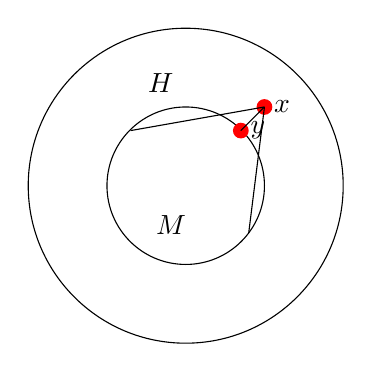
\begin{tikzpicture}
		\draw (0,0) circle(2);
		\draw (0,0) circle(1);
		\fill[red](0.7,0.7) circle (.1);
		\node at (0.7,0.7) [right] {$y$};
		\node at (1.0,1.0) [right] {$x$};
		\fill[red](1.0,1.0) circle (.1);
		\node at (-0.6,1.3) [right] {$H$};
		\node at (-0.5,-0.5) [right] {$M$};
		\path [draw] (0.7,0.7)--(1.0,1.0);
		\path [draw] (-0.7,0.7)--(1.0,1.0);
		\path [draw] (0.8,-0.6)--(1.0,1.0);
	\end{tikzpicture}
	\end{itemize}
\end{definition}
\begin{theorem}
设H希尔伯特空间(完备内积+赋范),$M\subset H$是$\textbf{凸闭集}$,则对$\forall x\in H,\exists !y\in M,s.t.$y是M中的最佳逼近元.
\end{theorem}
\begin{proof}
\begin{description}
	\item[step1] 存在性.\\
	令\begin{equation*}
		\alpha =\underset{z\in M}{inf}\left \| x-z\right \|
	\end{equation*}
则$\exists \{y_n\} \subset M,s.t. \quad \left \| x-y_n\right \|\to \alpha (n\to \infty)$\begin{align*}
	M\textbf{凸}&\Rightarrow \frac{y_n+y_m}{2}\in M,\quad (n,m\in \mathbb{N})\\
	&\Rightarrow \left \| x-\frac{y_n+y_m}{2}\right \|\geqslant \alpha
\end{align*} 
利用中线公式:$\left \| x+y\right \|^2+\left \| x-y\right \|^2=2\left \| x\right \|^2+2\left \| y\right \|^2$得\begin{align*}
	\left \| y_n-y_m\right \|^2&=\left \| y_m-x+x-y_n\right \|^2=2\left \| y_m-x\right \|^2+2\left \| y_n-x\right \|^2-\left \| 2x-(y_n+y_m)\right \|^2\\
	&=2\left \| y_m-x\right \|^2+2\left \| y_n-x\right \|^2-4\left \| x-\frac{y_n+y_m}{2}\right \|^2\\
	&\leqslant 2\left \| y_m-x\right \|^2+2\left \| y_n-x\right \|^2-4\alpha^2 \to 0
\end{align*}
从而$\{y_n\}$为cauchy列\\
于是$\exists y \in H,s.t. \{y_n\}\to y$,又M是闭集,故$y\in M$
\item[step2] 唯一性.\\
设$y'\in M$也是x在M中的最佳逼近元,利用中线公式\begin{align*}
	0\leqslant \left \| y-y'\right \| ^2&=2\left \| y-x\right \|^2+2\left \| x-y'\right \|^2-4\left \| x-\frac{y+y'}{2}\right \|^2\\
	& \leqslant 2\alpha^2+2\alpha^2-4\alpha^2=0
\end{align*}
\end{description}
\end{proof}
\begin{theorem}
设M是希尔伯特空间H的$\textbf{闭子空间}$,则对$\forall x\in H,\exists !$正交分解\begin{equation*}
	x=y+z,\quad y\in M,z\in M^{\perp}
\end{equation*}
\end{theorem}
\begin{proof}
\begin{description}
	\item[step1] 存在性\\
	M是H的闭子空间$\Rightarrow$M是凸闭集$\Rightarrow \exists !y$是x在M中的最佳逼近元.\\
	记$\alpha =\left \| x-y\right \|$ ,对$\forall u\in M,\forall \lambda$,又$y+\lambda u\in M$,于是\begin{align*}
		\alpha^2&\leqslant \left \| x-(y+\lambda u)\right \|^2\\
		&=\left \| (x-y)-\lambda\right \|^2\\
		&\leqslant \left \| x-y\right \|^2-\overline{\lambda}(x-y,u)-\lambda(u,x-y)+\left | \lambda\right |^2\left \| u\right \|^2
	\end{align*}
取$\lambda=\frac{(x-y,u)}{\left \| u\right \|^2}$,由于$\left \| x-y\right \|=\alpha$,则\begin{equation*}
	\alpha^2\leqslant \alpha^2-\frac{\left | (x-y,u)\right |^2}{\left \| u\right \|^2}
\end{equation*}
从而$(x-y,u)=0$,于是根据u的任意性可知$(x-y)\perp M$,故$x=y+(x-y)$,其中y是x关于M的最佳逼近元.
\item[step2] 唯一性证明省略,容易验证.
\end{description}
\end{proof}
\begin{note}
下面我们从二维空间出发讨论这个定理,如图.
\begin{figure}
	\centering
	\includegraphics[width=12cm,height=5cm]{12}
\end{figure}
\end{note}
\begin{note}
$M\oplus M^{\perp },M\subset M$闭子空间,\\
取$dimM=n,x=y+\eta,y\in M,\eta\in M^(\perp)$
\begin{align*}
	y&=\sum_{j=1}^{n}(y,e_j)e_j\\
	&=\sum_{j=1}^{n}(x-\eta,e_j)e_j\\
	&=sun_{j=1}^{n}(x,e_j)e_j
\end{align*}
\end{note}
\begin{definition}[$\textbf{内积空间中的规范正交系}$]
\begin{description}
	\item[1.] \begin{itemize}
		\item $\textbf{规范正交系}\quad $设H是内积空间,$\{e_n\}_{n=1}^{\infty}\subset H$,满足$(e_m,e_n)=\left\{\begin{matrix}
			0\quad m\neq n\\ 
			1\quad m=n
		\end{matrix}\right.$
	\item $\textbf{x关于}\{e_n\}_{n=1}^{\infty}\textbf{第n个Fourier系数} \quad c_n=(x,e_n)$
	\end{itemize}
\item[2.] 各空间的规范正交系 
\begin{itemize}
	\item $L^2[0,\pi]:\{\frac{1}{\sqrt{2\pi}}\}e^{int}$
	\item $l^2:\{e_n\}$
\end{itemize}
\item[3.] $\textbf{Bessel不等式}:\mathscr{X}$是一个希尔伯特空间(内积+赋范+完备),$\{e_n\}_{n=1}^{\infty}$是规范正交系,则对$\forall x\in \mathscr{X}$,成立\begin{equation*}
	\sum_{n=1}^{\infty}\left | (x,e_n)\right |^2\leqslant \left \| x\right \|^2
\end{equation*}
pf:任给n,记$\{e_j\}_{j=1}^n$张成空间为$Span\{e_j\}_{j=1}^n$,令$y=\sum_{k=1}^{n}(x,e_k)e_k$\\
故有$x=y+z,y\perp z$\\
则$\left \| x\right \|^2=\left \| y\right \|^2+\left \| z\right \|^2$\\
从而$\left \| y\right \|^2\leqslant \left \| x\right \|^2$\\
即$\sum_{k=1}^{n}\left | (x,e_k)\right |^2\leqslant \left \| x\right \|^2$,令$n\to \infty$,可得证.
\end{description}
\end{definition}
\begin{theorem}[$\textbf{Bessel公式(封闭公式)}$]
	设H希尔伯特空间(内积+赋范+完备),$\{e_n\}$为规范正交系.$\{c_n\}\in l^2$,则$\exists x\in H,s.t.$\begin{equation*}
		c_n=(x,e_n) \quad  \left \| x\right \|^2=\sum_{n=1}^{\infty}\left | c_n\right |^2=\sum_{n=1}^{\infty}\left | (x,e_n)\right |^2
	\end{equation*}
\end{theorem}
\begin{note}
	二者之间的关系:\\
$x+\{e_j\}_{j=1}^{\infty}\Rightarrow \{c_j\}_{j=1}^{\infty}=\{(x,e_j)\}_{j=1}^{\infty}$(Fourier系数,之前的定义)\\
$x=\sum_{j=1}^{\infty}c_je_j \Leftarrow \{c_j\}_{j=1}^{\infty}+\{e_j\}_{j=1}^{\infty}$
\end{note}
\begin{proof}
\begin{description}
	\item[step1] 令$x_n=\sum_{k=1}^{n}c_ke_k$,则\begin{equation*}
		\left \| x_m-x_n\right \|^2=\left \| \sum_{k=n+1}^{m}c_ke_k\right \|^2=\sum_{k=n+1}^{m}\left | c_k\right |^2\to 0\quad (n,m \to \infty)
	\end{equation*}
故$\{x_n\}$是H中的cauchy列,由于H完备,则$\exists x \in H$,s.t.$\{x_n\} \to x$,即$x=\sum_{j=1}^{\infty}c_je_j$
\item[step2] \begin{equation*}
	(x,e_t)\xleftarrow[\textbf{内积的连续性}]{n\to \infty}(x_n,e_t)=\left\{\begin{matrix}
		0 \quad n<t \\ 
		c_t \quad n \geqslant t
	\end{matrix}\right.
\end{equation*}
故$\{c_n\}$是x的Fourier系数,即$c_n=(x,e_n)$.\begin{equation*}
	\left\{\begin{matrix}
		\left \| x_n\right \|^2=\sum_{k=1}^{n}\left | c_k\right |^2\\ 
		\{x_n\}\to x\Rightarrow \left \| x_n\right \|\to \left \| x\right \|
	\end{matrix}\right.\Rightarrow \left \| x\right \|^2=\sum_{k=1}^{\infty}\left | c_k\right |^2
\end{equation*}
\end{description}
\end{proof}
\begin{theorem}[$\textbf{同构定理}$]
设H是一个可分的希尔伯特空间(存在稠密的可列子集),设dim H=n,则\\
$\exists $等距同构:\begin{align*}
	T: & H\to \mathbb{R}^n\\
	& x \mapsto \{(x,e_j)\}_{j=1}^n
\end{align*}
其中$\{e_j\}_{j=1}^{\infty}$是H的规范正交系$\quad (\mathbb{R}^{\infty}=l^2)$\\
\end{theorem}
\begin{proof}
只看dim H$=\infty$的情况,因为$n<\infty$时可分是显然的.\\
\begin{description}
	\item[step1] 构造H中的$\{e_j\}_{j=1}^{\infty}$(Schmidt正交化方法)\\
	$\because H$可分\\
	$\therefore $有可列的稠子集$\{x_j\}_{j=1}^{\infty}$\\
	取$e_1=\frac{x_1}{\left \| x_1\right \|}$\\
	再取$e_2=\frac{x_2-(x_2,e1)e_1}{\left \| x_2-(x_2,e_1)e_1\right \|}$\\
	$\cdots$\\
	$e_j=e_j=\frac{ x_j-\sum_{k=1}^{j-1}(x_j,e_k)e_k}{\left \| x_j-\sum_{k=1}^{j-1}(x_j,e_k)e_k\right \|}$\\
	容易验证:$\{e_j\}_{j=1}^{\infty}$是标准正交基\\
	(先证明两两正交,再证每个元素都可以用$\{e_j\}_{j=1}^{\infty}$表示,正交即可说明表示是唯一的)
	\item[step2] 构造等距同构映射T(证明如上定义的T为单、满、线性、等距)\\
	\begin{itemize}
		\item $\textbf{单射}$:即证:$Tx=0 \Rightarrow x=0$\\
		$Tx=0\Rightarrow (x,e_j)=0,\forall j\Rightarrow x=0$
		\item $\textbf{满射}$:$\forall \{c_j\}_{j=1}^{\infty}\in l^2,\exists x\in H,s.t. Tx=\{c_j\}_{j=1}^{\infty}$(就是帕赛瓦尔公式的证明过程)
		\item $\textbf{等距}$:$\sum_{j=1}^{\infty}(\left | (x,e_j)\right |^2)^{1/2}=\left \| x\right \|_H=\left \| Tx\right \|_l$(帕赛瓦尔公式)
		\item $\textbf{线性}$:\begin{align*}
			T(\alpha x+\beta y&=\{(\alpha x+\beta y,e_j)\}_{j=1}^{\infty}\\
			&=\alpha\{(x,e_j)\}_{j=1}^{\infty}+\beta\{(x,e_j)\}_{j=1}^{\infty}\\
			&=\alpha Tx+\beta Ty
		\end{align*}
	\end{itemize}
\item[step3] T的定义是合理的\\
即证:$\forall x\in H,Tx\in l^2$\\
即证:$\sum_{j=1}^{\infty}\left | (x,e_j)\right |^2<\infty$\\
根据Bessel不等式即可得证.(注意不适用Bessel等式,因为这里x是提前知道的,等式成立是x由$\{c_j\}$构造出来的,可以理解成逆映射$T^{-1}$使Bessel等式成立)
\end{description}
\end{proof}
\begin{note}
从以上结论中得出两个定义:
\begin{definition}[$\textbf{完备}$]
设H是内积空间,$\{e_n\}\subset H$为规范正交系,若对$\forall x \in H$,成立\begin{equation*}
	\left \| x\right \|^2=\sum_{n=1}^{\infty}\left | (x,e_n)\right |^2
\end{equation*}
则称$\{e_n\}$完备.
\end{definition}
\begin{definition}[$\textbf{完全}$]
设H为内积空间,$\{e_n\}\subset H$为规范正交系,若$\forall x \in H,(x,e_n)=0,n=1,2,3,\cdots \Rightarrow x=\theta$,则称$\{e_n\}$完全.
\end{definition}
\end{note}
\begin{note}
“无穷意义下的足够多”.\\以上构造中,H不一定完备,$\{e_n\}$的构造未知.
\end{note}
\begin{theorem}
设H是希尔伯特空间,$\{e_n\}_{n=1}^{\infty}$是H上的一个规范正交系,则以下命题等价:\begin{enumerate}
	\item $\{e_n\}_{n=1}^{\infty}$为H的标准正交基\\
	(或者说,$\forall x\in H,x=\sum_{n=1}^{\infty}(x,e_n)e_n$,也就是右边的级数收敛到x)
	\item $\{e_n\}_{n=1}^{\infty}$是完备的
	\item 保持内积\\
	(即$\forall x,y \in H,(x,y)_H=\sum_{n=1}^{\infty}(x,e_n)\overline{(y,e_n)}$)
	\item $\{e_n\}_{n-1}^{\infty}$完全
\end{enumerate}
\end{theorem}
\begin{proof}
\begin{description}
	\item[$1.\Rightarrow 2.$] Bessel等式的证明过程
	\item[$2.\Rightarrow 1.$] $\forall x \in H$,有\begin{align*}
		\left \| x-\sum_{k=1}^{n}(x,e_k)e_k\right \|^2&=( x-\sum_{k=1}^{n}(x,e_k)e_k, x-\sum_{k=1}^{n}(x,e_k)e_k)\\
		&=\left \| x\right \|^2-\sum_{k=1}^{n}(x,e_k)(e_k,x)-\sum_{k=1}^n \overline{(x,e_k)}(x,e_k)+\sum_{n=1}^n\left | (x,e_k)\right |^2\\
		&=\left \| x\right \|^2-\sum_{k=1}^{n}\left | (x,e_k)\right |^2\to 0
	\end{align*}
于是有$\sum_{k=1}^{\infty}(x,e_k)e_k\to x(n\to \infty)$,即$x=\sum_{k=1}^{\infty}(x,e_k)e_k.$
\item[$1.\Rightarrow 3.$] 由1.知\begin{align*}
	&\sum_{k=1}^{n}(x,e_k)e_k\to x\\
	&\sum_{k=1}^{n}(y,e_k)e_k\to y\\
	&(\sum_{k=1}^{n}(x,e_k)e_k,\sum_{k=1}^{n}(y,e_k)e_k)=\sum_{k=1}^{n}(x,e_k)(e_k,y)
\end{align*}
由内积的连续性\begin{equation*}
	\sum_{k=1}^{n}(x,e_k)(e_k,y)\to (x,y)
\end{equation*}
即\begin{equation*}
(x,y)=\sum_{k=1}^{n}(x,e_k) \overline{(y,e_k)}
\end{equation*}
\item[$3.\Rightarrow 4$] $(x,e_n)=0 \quad 1,2,\cdots \Rightarrow (x,x)=\sum_{n=1}^{\infty}(x,e_n)(e_n,x)=0\Rightarrow x=\theta$
\item[$4.\Rightarrow 2.$] 把$\{c_n\}_{n=1}^{\infty}=\{(x,e_n)\}_{n=1}^{\infty}$构造一个系数列,对$\forall x\in H$,令$y_n=\sum_{k=1}^{n}(x,e_k)e_k$,则在希尔伯特空间条件下,$\exists y\in H,s.t.\{y_n\}\to y$.\\
从而$\{(x,e_n)\}_{n=1}^{\infty}$是y关于$\{e_n\}_{n=1}^{\infty}$的Fourier系数\\
同时$\{(x,e_n)\}_{n=1}^{\infty}$也是x关于$\{e_n\}_{n=1}^{\infty}$的Fourier系数
\end{description}
故x-y的Fourier系数为0,即$(x-y,e_k)=0,k=1,2,\cdots \Rightarrow x-y=0 $\\
即$\left \| x-\sum_{k=1}^{\infty}(x,e_k)e_k\right \|=0$\\
即$\left \| x-\sum_{k=1}^{n}(x,e_k)e_k\right \|\to 0$\\
$\Rightarrow \left \| x\right \|^2-\sum_{k=1}^{n}\left | (x,e_k)e_k\right |^2\to 0$\\
$\Rightarrow \left \| x\right \|^2=\sum_{k=1}^{\infty}\left | (x,e_k)e_k\right |^2$
\end{proof}
\chapter{巴拿赫空间上的有界线性算子}
\begin{note}
\begin{equation*}
	\textbf{线性算子的问题}\left\{\begin{matrix}
		\textbf{基本概念(有界与连续,算子范数)}\\ 
		\textbf{所有有界线性算子的空间}\\ 
		\textbf{四个基本定理}\\ 
		\textbf{对偶空间,对偶算子;弱拓扑}\\ 
		\textbf{谱(有限维空间的特征值)}\\ 
		\textbf{紧算子}
	\end{matrix}\right.
\end{equation*}
\end{note}
\section{有界线性算子}
\begin{definition}
	\begin{itemize}
		\item $\textbf{可加}\quad $ T(x+y)=T(x)+T(y)
		\item $\textbf{齐次} \quad T(\alpha x)=\alpha T(x)$ 
		\item $\textbf{线性算子}\quad $可加齐次的映射
		\item $\textbf{泛函}\quad T:D\subset \mathscr{Z}\to \mathbb{R}/\mathbb{C}$
		\item $\textbf{线性泛函}\quad$ 线性+泛函
		\item $\textbf{连续线性算子}\quad T$连续
		\item $\textbf{有界线性算子}\quad $T将D中有界$\overset{\textbf{映成}}{\rightarrow}$有界
		\item $\textbf{无界线性算子} \quad $T将D中有界$\overset{\textbf{映成}}{\rightarrow}$无界
	\end{itemize}
\end{definition}
\begin{note}
	\begin{enumerate}
		\item T连续$\Leftrightarrow $T将$\mathscr{X}$中cauchy列$\overset{\textbf{映成}}{\rightarrow}\mathscr{Y}$中cauchy列
		\item T有界$\Leftrightarrow $T将D中有界$\overset{\textbf{映成}}{\rightarrow}$有界
		\item 线性与连续的关系:\begin{equation*}
			\textbf{T连续}\Rightarrow \left\{\begin{matrix}
				\textbf{若}k=\mathbb{R},\textbf{T可加}\Rightarrow \textbf{T齐次}\\ 
				\textbf{若}k=\mathbb{C},\textbf{T可加}+T(ix)=iTx \Rightarrow \textbf{T齐次}
			\end{matrix}\right.
		\end{equation*}
	\end{enumerate}
\end{note}
\begin{theorem}
设$\mathscr{Z},\mathscr{Y}$均为赋范空间,$T:\mathscr{Z}\to \mathscr{Y}$为线性的,则以下等价:\begin{description}
	\item[1.] T在$\mathscr{Z}$中某点连续
	\item[2.] T连续
	\item[3.] T有界
	\item[4.] $\exists M \geqslant 0,s.t. \left \| Tx\right \|_{\mathscr{Y}}\leqslant M\left \| x\right \|_Z,\forall X\in \mathscr{X}$
\end{description}
\end{theorem}
\begin{proof}
\begin{figure}
	\centering
	\includegraphics[width=19cm,height=20cm]{13}
\end{figure}
\end{proof}
\begin{note}
在线性同构条件下:范数等价同构 $\Leftrightarrow $拓扑同构$\quad \left \| Tx-Ty\right \|=\left \| x-y\right \|\Leftrightarrow T,T^{-1}$连续.
\end{note}
\begin{definition}[$\textbf{T的范数}$]
$\left \| T\right \|\overset{\triangle }{=}inf\{M|\left \| Tx\right \|\leqslant M\left \| x\right \|,\forall x\in \mathscr{X}\}$
\end{definition}
\begin{note}
\begin{itemize}
	\item $\left \| Tx\right \|\leqslant \left \| T\right \|\left \| x\right \|,\quad \forall x\in \mathscr{X}$
	\item $\left \| Tx\right \|=\underset{0\neq x\in \mathscr{X}}{sup}\frac{\left \| Tx\right \|}{\left \| x\right \|}=\underset{\left \| x\right \|=1,x\in \mathscr{X}}{sup}\left \| Tx\right \| $
	\item 例子:\begin{description}
		\item[1)] $T:\mathbb{R}^n\to \mathbb{R}^n\quad , x \mapsto Ax$线性\\
		$\left \| Tx\right \|=\left \| Ax\right \|\leqslant (\sum_{1\leqslant i,j\leqslant n}a_{ij}^2)^{1/2}\left \| x\right \|$\\
		$\Rightarrow \left \| T\right \|\leqslant (\sum_{1\leqslant i,j\leqslant n}a_{ij}^2)^{1/2}$
		\item[2)] $T:C[a,b]\to C\quad ,x(t)\mapsto \int_{a}^{b}x(t)dt$\\
		$\left | Tx\right |=\left | \int_{a}^{b}x(t)dt\right |\leqslant (b-a)\left \| x\right \| $\\
		$\Rightarrow \left \| T\right \|\leqslant (b-a)$
		\item[3)] $T:C[a,b]\to C[a,b]\quad ,x(t)\mapsto \int_{a}^{b}K(t,s)x(s)ds,K(t,s)\in C^2[a,b]\times[a,b]$\\
		则T是有界线性算子,且$\left \| x\right \|=\underset{a\leqslant t\leqslant b}{max}\int_{a}^{b}\left | K(t,s)\right |ds$\\
		pf:\begin{align*}
			 \left \| Tx\right \|&=\underset{a\leqslant t\leqslant b}{max}\left | \int_{a}^{b}K(t,s)x(s)ds\right |\\
			 &\leqslant \underset{a\leqslant t\leqslant b}{max}\left | x(t)\right |\cdot \underset{a\leqslant t\leqslant b}{max}\int_{a}^{b}\left | K(t,s)\right |ds\\
			 &\overset{\triangle }{=}\alpha \left \| x\right \|
		\end{align*}
		$\Rightarrow T$有界且$ \left \| T\right \| \leqslant \alpha.$\\
		又$\int_{a}^{b}\left | K(t,s)\right |ds$关于t连续,则$\exists t_0\in [a,b],s.t.$\begin{equation*}
			\alpha =\int_{a}^{b}\left | K(t_0,s)\right |ds
		\end{equation*}
\begin{align*}
		\varphi_n(t)&=\frac{1-nd(t,e_0)}{1+nd(t,e_0)},\quad e_0=\{s:K(t_0,s)\geqslant 0\}\\
		&=\left\{\begin{matrix}
			1& K(t_0,t)\geqslant 0\\ 
			\frac{\frac{1}{n}-d(t,e_0)}{\frac{1}{n}+d(t,e_0)}\to -1&(n\to \infty)
		\end{matrix}\right.
\end{align*}
\begin{align*}
	(T\varphi_n)(t_0)&=\int_{a}^{b}K(t_0,s)\varphi_n(s)ds\\&\xrightarrow[\textbf{分成两部分,大于等于0的部分不变,小于0的部分}\to \int \left |\cdot \right |]{DCT}\int_{a}^{b}\left | K(t_0,s)\right |ds=\alpha
\end{align*}
\\
$\Rightarrow \alpha=\underset{n\to \infty}{lim}\left | (T\varphi)(t_0)\right |\leqslant \underset{n\to \infty}{lim}\left \| T\varphi_n\right \|\leqslant \underset{n\to \infty}{lim}\left \| T\right \|\cdot \left \| \varphi_n\right \|=\left \| T\right \|$\\
从而$\alpha =\left \| T\right \|$
\item[4)] T:$C[a,b]\to C[0,1]\quad, x(t)\mapsto \frac{d}{dt}x(t)$\\
(max$\left | x'-y'\right |$与$max\left | x-y\right |$没有关系。)\\
pf:$\quad $令$x_n(t)=\sin nt$,则$\left \| x_n(t)\right \|=1$\\
但$\left \| Tx_n\right \|=n\left \| \cos nt\right \|=n\to \infty\quad(n\to \infty)$\\
把单位球面$\overset{\textbf{映成}}{\rightarrow}$无界集.
	\end{description}
\end{itemize}
\end{note}
\section{有界线性算子空间}
\begin{definition}
	 设$\mathscr{X},\mathscr{Y}$均为赋范空间,\\
	 记$B(\mathscr{X},\mathscr{Y})=\{T|T:\mathscr{X}\to \mathscr{Y}\textbf{为有界线性算子}\}$,\\
	 $B(\mathscr{X},\mathscr{X})\overset{\triangle }{=}B(\mathscr{X})$\\
 空间$B(\mathscr{X},\mathscr{Y})$按算子范数可以构成一个有界线性算子空间.
\end{definition}
\begin{proof}
\begin{figure}
	\centering
	\includegraphics[width=19cm,height=20cm]{14}
\end{figure}
\end{proof}
\begin{definition}[$\textbf{按算子范数收敛(一致算子拓扑)}$] $\left \| T_n-T\right \|\to 0\quad (n\to \infty)$
\end{definition}
\begin{theorem}
$\{T_n\},T\in B(\mathscr{X},\mathscr{Y})$,则$T_n$按一致算子拓扑收敛于T$\Leftrightarrow T_n$在任意有界集上一致收敛于T.
\end{theorem}
\begin{proof}
\centering
\includegraphics[width=19.5cm,height=16cm]{15}
\end{proof}
\begin{note}
$\left\{\begin{matrix}
	\textbf{一致算子拓扑}\\ 
	\textbf{强算子拓扑}\\ 
	\textbf{弱拓扑}
\end{matrix}\right.$\\
$\textbf{算子的强拓扑}$:对每个$x\in \mathscr{X}$,有$\underset{n\to \infty}{lim}\left \| T_nx-Tx\right \|=0$\\
$T_n \overset{S}{\rightarrow}T\Leftrightarrow \forall x\in \mathscr{X},T_nx\to Tx(n\to \infty)$\\
\end{note}
\begin{note}
例子:强收敛但不一致收敛\\
定义$l^p$上的算子:$T_n \xi=\xi_n,\xi=\{x_j\}_{j=1}^{\infty},\xi_n=\{x_j\}_{j=n}^{\infty}$\\
则$T_n\in B(l^p,l^p)=B(l^p)$\\
\begin{enumerate}
	\item 显然:$\left \| T_n\xi\right \|=\left ( \sum_{j=n}^{\infty}\left | x_j\right |^p\right )^{1/p}\leqslant \left ( \sum_{j=1}^{\infty}\left | x_j\right |^p\right )^{1/p}=\left \| \xi\right \|$\\
	$\Rightarrow \left \| T_n\right \|\leqslant 1$\\
	取$\xi_0=\{0,\cdots,x_n,x_{n+1},\cdots\}\in l^p$,则$T_n\xi_0=\xi_0$\\
	$\Rightarrow \left \| T_n\right \|\geqslant 1$\\
	从而$\left \| T_n\right \|=1,\quad n=1,2,\cdots$
	\item 但$\left \| T_n\xi\right \|=\left(\sum_{j=n}^{\infty}\left | x_j\right |^p\right)^{1/p}\to 0(n\to \infty)$,即$T_n\overset{s}{\rightarrow}0$\\
	T一致收敛于1,强收敛于0.
\end{enumerate}
\end{note}
\begin{theorem}
\begin{enumerate}
\item $B(\mathscr{X},\mathscr{Y})$在一致拓扑收敛下完备$\Leftarrow \mathscr{Y}$完备
\item $B(\mathscr{X},\mathscr{Y})$在强算子拓扑下完备$\Leftarrow \mathscr{X},\mathscr{Y}$完备
\end{enumerate}
\end{theorem}
\begin{proof}
	\centering
	\includegraphics[width=19cm,height=20cm]{17}
\end{proof}
\begin{definition}[$\textbf{算子的乘法}$]$\mathscr{X},\mathscr{Y}$为赋范线性空间,定义如下乘法运算:
$\mathscr{X}\overset{T}{\rightarrow}\mathscr{Y}\overset{S}{\rightarrow}\mathscr{X}$\\
$ST:\mathscr{X}\to \mathscr{X}\quad (ST)x=S(Tx)$\\
\end{definition}
\begin{note}
\begin{itemize}
	\item $\mathscr{X},\mathscr{Y}$为线性空间:$T,S$线性$\Rightarrow $ST线性
	\item $\mathscr{X},\mathscr{Y}$为赋范空间:$T,S$有界$\Rightarrow$ ST有界\begin{align*}
		\left \| (ST)x\right \|_{\mathscr{X}}&=\left \| S(Tx)\right \|_{\mathscr{X}}\\
		&\leqslant \left \| S\right \|\left \| Tx\right \|\\
		&\leqslant \left \| S\right \|_{B(\mathscr{Y},\mathscr{X})}\left \| T\right \|_{B(\mathscr{Z},\mathscr{Y})}\left \| x\right \|_{\mathscr{Z}}
	\end{align*}
故ST有界,从而$ST\in B(\mathscr{X},\mathscr{Y})$
\item 乘法满足分配律、结合律
\item $S,T\in B(\mathscr{X})$,S,T不一定可交换,即$ST\neq TS$
\end{itemize}
\end{note}
\section{四个基本定理}
四个基本定理\begin{equation*}
	\left\{\begin{matrix}
		\textbf{开映射定理(连续映射定理)}\\ 
		\textbf{闭图像定理}\\ 
		\textbf{共鸣定理}\\ 
		\textbf{泛函的延拓定理}
	\end{matrix}\right.
\end{equation*}
\begin{theorem}[$\textbf{开映射定理}$]
设T$\in B(\mathscr{X},\mathscr{Y})$,$\mathscr{X},\mathscr{Y}$均为Banach空间,则\begin{equation*}
	D(T)=\left\{\begin{matrix}
		\textbf{一型集}\subset \mathscr{Y}\\ 
		\textbf{二型集}=\mathscr{Y},\textbf{且}\forall y\in \mathscr{Y},\exists x\in \mathscr{X},s.t. \quad Tx=y,\left \| x\right \|\leqslant K\left \| Tx\right \|
	\end{matrix}\right.
\end{equation*}	
\end{theorem}
\begin{note}
二型集:不可表示为至多可列个稀疏集;\\
由定理知,若D(T)=$\mathscr{Y}$,则T是单射;\\
但是T不一定是可逆的;若T可逆,则由定理21的等价性质,可知,$T^{-1}$有界.
\end{note}
\begin{proof}
\centering
\includegraphics[width=16cm,height=20cm]{18}
\centering
\includegraphics[width=18cm,height=20cm]{19}
\end{proof}
\begin{theorem}[$\textbf{逆算子定理}$]
设$T\in B(\mathscr{X},\mathscr{Y}),\mathscr{X},\mathscr{Y}$均为Banach空间,且T为双射,则$T^{-1}\in B(\mathscr{Y},\mathscr{X})$.
\end{theorem}
\begin{note}
只需要看它的拓扑性,代数性很自然
\end{note}
\begin{proof}
	D(T)=$\mathscr{Y}$\\
	$\left \| T^{-1}y\right \|=\left \| x\right \|\leqslant K\left \| Tx\right \|=K\left \| y\right \|$\\
	故$T^{-1}$有界.
\end{proof}
\begin{theorem}[推论]
设$(\mathscr{X},\left \| \cdot \right \|_1),(\mathscr{Y},\left \| \cdot \right \|_2)$均为Banach空间,若$\exists K,s.t.$,对于$\forall x\in \mathscr{X}$,有\begin{equation*}
	\left \| x\right \|_2\leqslant K\left \| x\right \|_1
\end{equation*}
则$(\mathscr{X},\left \| \cdot \right \|_1),(\mathscr{Y},\left \| \cdot \right \|_2)$拓扑同构.
\end{theorem}
\begin{proof}
I:$\quad (\mathscr{X},\left \| \cdot \right \|_1)\to (\mathscr{X},\left \| \cdot \right \|_2)\quad x \mapsto x$\\
I是双射,$ \quad$ 则$ \left \| x\right \|_2\leqslant K \left \| x\right \|_1$,$\quad $故I有界.\\
则$I\in B(\mathscr{X},\mathscr{X})$, \\
从而由逆算子定理可知:$\quad I^{-1}\in  B(\mathscr{X},\mathscr{X})$,\\
故$(\mathscr{X},\left \| \cdot \right \|_1),(\mathscr{Y},\left \| \cdot \right \|_2)$等价.
\end{proof}
\begin{definition}
设T:D(T)$\subset \mathscr{X}\to \mathscr{Y}$线性\\
\begin{itemize}
	\item $\textbf{T的图像}:G(T)\overset{\triangle }{=}\left \{(x,Tx)|x\in D(T)\right \}\subset \mathscr{X}\times \mathscr{Y}$
	\item $\textbf{T为闭算子}:$若$G(T)\subset \mathscr{X}\times \mathscr{Y}$为闭子空间.
\end{itemize}
\end{definition}
\begin{theorem}
以下性质等价:\begin{enumerate}
	\item T闭
	\item $\forall D(T) \ni x_n \to x,\quad Tx_n\to y$,则$x\in D(T)$,且$Tx=y$
	\item $^*$(前提:$\mathscr{X} ,\mathscr{Y}$完备) $\left [ D(T)\right ]=\left ( D(T),\left \| x\right \|+\left \| Tx\right \|\right )$
\end{enumerate}
\end{theorem}
\begin{proof}
\centering
\includegraphics[width=14cm,height=13.5cm]{20}
\end{proof}
\begin{theorem}[$\textbf{闭图像定理}$]
	设$\mathscr{X},\mathscr{Y}$为Bananch空间,$T\in B(\mathscr{X},\mathscr{Y})$,则T为闭算子$\Leftrightarrow $T有界
\end{theorem}
\begin{proof}
\centering
\includegraphics[width=14cm,height=17cm]{21}
\end{proof}
\begin{note}
\begin{itemize}
	\item 若D(T)只是$\mathscr{X}$子空间,则闭算子不一定有界
	\item $D(T)\subset \mathscr{X}$是稠子集,则$\overline{D(T)}=\mathscr{X}$
	\item 例:
	\begin{align*}
		T:      &C^1[a,b] \to C[a,b]\\
		        &f \mapsto \frac{d}{dt}
	\end{align*}
$C^1[a,b]\ni \{x_n\}\to x\in C[a,b],\quad \{x'_n\}\to y\in C[a,b]$\\
即$\left\{\begin{matrix}
	x_n\overset{\textbf{一致}}{\rightarrow}x\\ 
	x'_n\overset{\textbf{一致}}{\rightarrow}y
\end{matrix}\right. \Rightarrow x'=y$即$Tx=y.$\\
从而T是闭算子,但是显然T不有界.
\end{itemize}
\end{note}
\begin{theorem}[$\textbf{共鸣定理}$]
设$\{T_{\lambda}\}_{\lambda\in \Lambda }\subset B(\mathscr{X},\mathscr{Y})$,$\mathscr{X}$为Banach空间,则$\{T_{\lambda}\}$强有界$\Rightarrow\{T_{\lambda}\}$有界(一致有界)
\end{theorem}
\begin{proof}
\centering
\includegraphics[width=14cm,height=17cm]{22}
\end{proof}
\begin{theorem}[$\textbf{泛函的延拓定理}$]
设$\mathscr{X}$为赋范线性空间,$\mathscr{X}_0$是$\mathscr{X}$的子空间,则$\forall x_0^*\in \mathscr{X}_0^*,\exists x^*\in \mathscr{X}^*$,使\begin{equation*}
	x^*|_{\mathscr{X}_0}=x_0^*,\quad \left \| x^*\right \|_{\mathscr{X}^*}=\left \| x_0^*\right \|_{\mathscr{X}_0^*}
\end{equation*}
\end{theorem}
\begin{proof}
	证明先放一放,自己去看吧,好多...
\end{proof}
\begin{note}
\begin{itemize}
	\item 设G是赋范线性空间E的子空间,$x_0\in E\setminus G$,若\begin{equation*}
		d(x_0,G)=\underset{x\in G}{inf}\left \| x_0-x\right \|=\delta >0
	\end{equation*}
则$\exists f \in E^*$,使$\left \| f\right \|=\frac{1}{\delta},\quad f(x_0)=1$
\item  设G是赋范线性空间E的子空间,$x_0\in E\setminus G$,若\begin{equation*}
	d(x_0,G)=\underset{x\in G}{inf}\left \| x_0-x\right \|=\delta >0
\end{equation*}
则$\exists f \in E^*$,使$\left \| f\right \|=1,\quad f(x_0)=\delta$
\item 设$A\subset \mathscr{X}$,取$\mathscr{X}_0=span A$\\
$x_0$可由A的元素的线性组合逼近($x_0\in \overline{span A}$)$\Leftrightarrow \forall x^*\in \mathscr{X}^*$,若$x^*|_A=0$,则$\left \langle x^*,x_0\right \rangle=0$
\item 任给$0\neq x_0\in \mathscr{X},\exists x^*\in \mathscr{X}^*$,使$\left \| x^*\right \|=1$,且$\left \langle x^*,x_0\right \rangle=\left \| x_0\right \|$
\item 延拓不唯一,且构成的集合不小于阿列夫零
\end{itemize}
\end{note}
\section{对偶空间与伴随算子}
\begin{definition}[$\textbf{对偶空间}$]
$\mathscr{X}$上的所有有界线性泛函(映射到实数或复数域)构成的赋范线性空间称为$\mathscr{X}$的赋范空间.
\end{definition}
\begin{note}
其上定义的线性运算如下:\begin{equation*}
	\left \langle \alpha x^*+\beta y^*,x\right \rangle=\alpha \left \langle x^*,x\right \rangle+\beta \left \langle y^*,x\right \rangle
\end{equation*}
范数:\begin{equation*}
	\left \| y^*\right \|=\underset{x\neq \theta ,x\in \mathscr{X}}{sup}\frac{\left | f(x)\right |}{\left \| x\right \|}
\end{equation*}
\end{note}
\begin{theorem}[$\textbf{嵌入定理}$]
设$\mathscr{X}$为一个赋范空间,则$\mathscr{X}\xrightarrow[]{\textbf{等距嵌入}}\mathscr{X}^{**}$
\end{theorem}
\begin{proof}
\centering
\includegraphics[width=14cm,height=12cm]{23}
\end{proof}
\begin{note}
\begin{itemize}
	\item $x\mapsto x^{**}\quad $,若满射,则称$\mathscr{X}$为$\textbf{自反空间}$.
	\item $\tau $具体化不一定.
\end{itemize}
例子:\begin{itemize}
	\item 空间$C[a,b]$的对偶空间\\
	设f为$C[a,b]$上的有界线性泛函,则$\exists $有界线性变差函数v$\in [a,b]^*$,s.t.对一切x$\in C[a,b]$,有\begin{equation*}
		f(x)=\int_{a}^{b}x(t)dv(t)
	\end{equation*}
且$\overset{b}{\underset{a}{V}}(v)=\left \| f\right \|$,这里$\overset{b}{\underset{a}{V}}(v)$表示v在$[a,b]$上的全变差.
\item 空间$L^p[a,b]$的对偶空间使$L^q[a,b]$
,这里$\frac{1}{p}+\frac{1}{q}=1$
\end{itemize}
\end{note}
\begin{definition}[$\textbf{伴随算子}$]
设$T\in B(\mathscr{X},\mathscr{Y})$,定义$T^*\in B(\mathscr{Y}^*,\mathscr{X}^*)$\begin{equation*}
	\left \langle T^*y^*,x\right \rangle\overset{\triangle }{=}\left \langle y^*,Tx\right \rangle
\end{equation*}
\end{definition}
\begin{note}
性质\begin{itemize}
	\item 可定义\\
	(就是证明$T^*y^*$是一个有界线性算子)
	\item $T^*$线性\\
	(就是证明$\left \langle T^*(\alpha x^*+\beta y^*),x\right \rangle=\alpha \left \langle T^*x^*,x\right \rangle+\beta \left \langle T^*y^*,x\right \rangle$)
	\item $T^*$有界\\
	$\left | \left \langle T^*,y^*,x\right \rangle\right |=\left | y^*(Tx)\right |\leqslant \left \| y^*\right \|\cdot \left \| T\right \|\cdot \left \| x\right \|$\\
	$\Rightarrow \left \| T^*\right \|\leqslant \left \| T\right \|\cdot \left \| y^*\right \|$\\
	故$\left \| T^*\right \|$有界且$\left \| T^*\right \|\leqslant \left \| T\right \|$\\
	另一方面,有哈恩——巴拿赫定理的推论知\\
	$\forall x\in \mathscr{X},\exists y^*\in \mathscr{Y}^*$,s.t.$\left | \left \langle y^*,Tx\right \rangle\right |=\left \| Tx\right \|,\quad \left \| y^*\right \|=1$\\
	从而$\left \| Tx\right \|=\left | \left \langle y^*,Tx\right \rangle\right |=\left | \left \langle T^*y^*,x \right \rangle\right |\leqslant \left \| T^*\right \|\cdot \left \| y^*\right \|\cdot \left \| x\right \|$
	$\Rightarrow \left \| T\right \|\leqslant \left \| T^*\right \|$\\
	综上$\left \| T\right \|= \left \| T^*\right \|$
\end{itemize}
\end{note}
\begin{theorem}
$*:B(\mathscr{X},\mathscr{Y})\to B(\mathscr{Y}^*,\mathscr{X}^*),\quad T\mapsto T^*$,满足
	\begin{enumerate}
		\item *是等距的
		\item $(\alpha T+\beta S)^*=\alpha T^*+\beta S^*$
		\item $(ST)^*=T^*S^*$
		\item $T^{**}=(T^*)^*$是T的延拓
		\item $T^{-1} \in B(\mathscr{Y},\mathscr{X})\Leftrightarrow (T^*)^{-1}\in  B(\mathscr{X}^*,\mathscr{Y}^*)$\\
		设$\mathscr{X},\mathscr{Y}$均为Banach空间,此时$(T^{-1})^*=(T^*)^{-1}$
	\end{enumerate}
\end{theorem}
\begin{proof}
我们只证明4和5
\centering
\includegraphics[width=14cm,height=17cm]{24}
\end{proof}
\begin{definition}[$\textbf{弱*收敛}$]
	$\{x_n^*\}\subset \mathscr{X}^*,\quad x_0^*\in \mathscr{X}^*$\begin{equation*}
		x_n^*\xrightarrow[]{w^*}x_0^*\Leftrightarrow \left \langle x_n^*,x\right \rangle\to \left \langle x_0^*,x\right \rangle
	\end{equation*}
\end{definition}
\begin{note}
性质:\begin{itemize}
	\item 极限唯一
	\item $\mathscr{X}^*$中的范数拓扑收敛$\Rightarrow \mathscr{X}^*$中的$w^*$拓扑收敛\\
	$\left | x^*_n(x)-x_0^*(x)\right |\leqslant \left \| x_n^*-x\right \|\cdot \left \| x\right \|\to 0$
\end{itemize}
\end{note}
\begin{note}
总结:\begin{equation*}
	\textbf{赋范线性空间}\left\{\begin{matrix}
		\textbf{点列的范数拓扑}:\textbf{按范数收敛}\\ 
		\textbf{有界线性算子拓扑}\left\{\begin{matrix}
			T_n\overset{s}{\rightarrow}T\quad \textbf{按强算子拓扑收敛}\\ 
			T_n\to T\quad \textbf{按一致算子拓扑收敛}
		\end{matrix}\right.
	\end{matrix}\right.
\end{equation*}
\begin{equation*}
	\textbf{对偶空间}\left\{\begin{matrix}
		\textbf{弱*收敛}\quad T_n\overset{w^*}{\rightarrow}T\\ 
		\textbf{弱收敛}\quad T_n\overset{w}{\rightarrow}T
	\end{matrix}\right.
\end{equation*}
\end{note}
\begin{theorem}
	设$\mathscr{X}$是Banach空间,$\{f_n\}\subset \mathscr{X}^*$,则$f_n\overset{w^*}{\rightarrow}f$\\
	$\Leftrightarrow $\begin{itemize}
		\item $\{f_n\}$一致有界
		\item $\forall x\in G\subset \mathscr{X}$,稠密子集,$\{f_n(x)\}$收敛
	\end{itemize}
\end{theorem}
\begin{definition}[$\textbf{弱收敛}$]
$\mathscr{X}\ni x_n\overset{w}{\rightarrow} x_0\in \mathscr{X}\Leftrightarrow \left \langle x^*,x_n\right \rangle\to \left \langle x^*,x\right \rangle,\quad \forall x^*\in \mathscr{X}^*$
\end{definition}
\begin{note}
性质:\begin{enumerate}
	\item $x_n\overset{\textbf{一致}}{\rightarrow} x \Rightarrow x_n\overset{w^*}{\rightarrow}x$
	\item 收敛极限唯一
	\item $x_n\overset{w^*}{\rightarrow}x \Rightarrow \underset{n}{sup}\left \| x_n\right \|<\infty$(这个证明蛮不错的,回去书上看看,构造$\mathscr{X}\to \mathscr{X}^*$的典范嵌入)
\end{enumerate}
\end{note}
\begin{note}
例子:\begin{enumerate}
	\item $\mathscr{X}=C[0,1],x,x_n\in \mathscr{X}$\\
	$x_n\to x \Leftrightarrow $上确界范数收敛$\Leftrightarrow $一致收敛\\
	$x_n\overset{w}{\rightarrow}x \Leftrightarrow  \underset{n}{sup}\left \| x_n\right \|<\infty$且逐点收敛
	\item $x_n\to x\Rightarrow x_n\overset{w}{\rightarrow}x\Rightarrow $逐点收敛\\
	但是反过来的充分条件两个都不成立,反例如下:\\
	\begin{enumerate}
	\item $x_n(t)=\frac{1}{nt}$逐点$\to 0$,但$x_n$不$\overset{w}{\rightarrow}$0,因为$x_n(0)\to \infty$不是一致有界的(前面的等价定理)
	\item $x_n=\frac{nt}{1+n^2t^2}\quad 0\leqslant t \leqslant 1$,逐点收敛到0,但在对偶空间上不会强收敛到0\\
	(这里的强收敛是在对偶空间里的强收敛,不是实数域上的强收敛,注意区别,因为在对偶空间上的强收敛实际对应的是赋范线性空间空间上的一致收敛,而对偶空间上的弱*收敛对应赋范线性空间上的强收敛,所以说强收敛强于弱*收敛和弱收敛).\\
	$\left \| x_n(t)\right \|\leqslant \frac{1}{2}$,又$t=\frac{1}{n}$时,$\left \| x_n(t)\right \|= \frac{1}{2}$,故$x_n\to \frac{1}{2}$,但是$x_n(t)\overset{w}{\rightarrow}0$
	\end{enumerate}
	\item $\mathscr{X}=L^p[0,1]\quad (1<p<\infty)$\\
	$x_n\overset{w}{\rightarrow}x\Leftrightarrow \underset{n}{sup}\left \| x_n\right \|_{L^p}<\infty$且$\forall t\in [0,1],\quad \int_{0}^{t}x_n(s)ds\to \int_{0}^{t}x(s)ds$
	(注意:$L^p[0,1]\subset L[0,1]$)(证明省略,自己去看书吧,好长)
\end{enumerate}
注意:上面的没有标注的收敛都是强收敛.\\
第一个例子的证明如下:
\centering
\includegraphics[width=14cm,height=17cm]{25}

\end{note}
\begin{theorem}[$\textbf{三种收敛之间的关系}$]
	$T_n,T\in B(\mathscr{X},\mathscr{Y})$
\begin{enumerate}
	\item 一致算子拓扑收敛:$T_n\overset{u}{\rightarrow}TT_n\overset{u}{\rightarrow}T\Leftrightarrow \left \| T_n-T\right \|\to 0$
	\item 强算子拓扑:$T_n\overset{s}{\rightarrow}T\Leftrightarrow  \forall x\in \mathscr{X},\quad \left \| T_nx-Tx\right \|\to 0$
	\item 弱算子拓扑:$T_n\overset{w}{\rightarrow}T\Leftrightarrow \forall y^*\in \mathscr{Y}^*,\quad \left | \left \langle y^*,T_nx\right \rangle-\left \langle y^*,Tx\right \rangle\right |\to 0,\quad \forall x\in \mathscr{X}$(注意对x是一致的,因为$y^*$是作用在T上的)
\end{enumerate}
(补充一点:1、2所说的收敛是在赋范线性空间上的算子拓扑,而3所说的弱收敛是在对偶空间上的算子拓扑,一定要分清楚)
\end{theorem}
\section{有界线性算子的正则集与谱}
\begin{definition}[$\textbf{可逆}$]
$T\in B(\mathscr{X},\mathscr{Y})$既是单映射又是满映射,则T的逆算子$T^{-1}$存在,当T存在逆算子时,称T是$\textbf {可逆的}$.\\
其中$T^{-1}T=I_{\mathscr{X}},TT^{-1}=I_{\mathscr{Y}}$,称$T^{-1}$是T的$\textbf{逆算子}$.
\end{definition}
\begin{note}
两个性质:\begin{itemize}
	\item 若T的逆算子存在,则有\begin{align*}
		TT^{-1}&=I_{\mathscr{Y}}\\
		T^{-1}T&=I_{\mathscr{X}}
	\end{align*}
\item 若$\exists S:\mathscr{Y}\to \mathscr{X},R(s)\subset\mathscr{X},\quad S_1:\mathscr{Y}\to \mathscr{X}\quad R(s_1)\subset \mathscr{X}$\\
s.t. $ST=I_{\mathscr{X}}$(左逆$\to$单射)\\
\qquad $TS_1=I_{\mathscr{Y}}$(右逆$\to$双射)\\
则T可逆,且$T^{-1}=S=S_1$
\end{itemize}
\end{note}
\begin{theorem}[$\textbf{逆算子定理} $]
	设$\mathscr{X},\mathscr{Y}$均是Banach空间,则\\
	t是有界逆算子$\Leftrightarrow T^*$有有界逆算子,且此时$(T^{-1})^*=(T^*)^{-1}$
\end{theorem}
\begin{proof}
	\centering
	\includegraphics[width=14cm,height=17cm]{26}
	\centering
	\includegraphics[width=15cm,height=10cm]{27}
\end{proof}
\begin{definition}
考虑$\textbf{预解式}$:$R(\lambda,T)\overset{\triangle }{=}\lambda-T\overset{\triangle }{=}\lambda I-T$.\\
\begin{itemize}
	\item T的预解集:$\rho(T)=\{\lambda\in\mathbb{C}|(\lambda-I)^{-1}\in B(\mathscr{X})\}$
\item T的点谱:$\sigma_p(T)=\{\lambda \in \mathbb{C}|\lambda-T\textbf{不是单射}\}$

\item T的连续谱:$\sigma_c(T)=\{\lambda\in \mathbb{C}| \lambda-T\textbf{是单射},R(\lambda-T)\textbf{是}\mathscr{Y}\textbf{的稠密子集}\}$
\item T的剩余谱:$\sigma_r(T)=\{\lambda \in \mathbb{C}|\lambda-T\textbf{是单射},\overline{R(\lambda-T)}\}\textbf{不是}\mathscr{Y}\textbf{稠密子集}$
\item 特征值:当$\lambda \in \sigma_p(T)$时,$(\lambda I-T)x=0$有非零解,$\lambda$称T的特征值.
\end{itemize}
\end{definition}
\begin{note}
$\sigma(T)=\sigma_p\cup \sigma_c\cup \sigma_r$,$\mathbb{C}=\rho(T)\cup\sigma(T)$
\end{note}
\begin{note}
例子:\begin{enumerate}
	\item  T$\in B(\mathbb{C}^n)\Rightarrow T=A_{n\times n},\quad \sigma\{A_{n\times n}\}=\{\lambda _j\}_{j=1}^n$(包括重数)\begin{equation*}
		\left\{\begin{matrix}
			\textbf{几何重数} \quad dim\quad ker(\lambda-T) \quad \textbf{特征子空间维数(Jordan块个数)}\\ 
			\textbf{代数重数} \quad dim \quad R(\lambda-T) \quad \textbf{Jordan块阶数之和}
		\end{matrix}\right.
	\end{equation*}
我们可以得出:$T^*=T\Rightarrow $几何重数=代数重数.\\
因为由之前的例题我们知道$A^*=A^T$,\\
故$T^*=T \Rightarrow A^T=A\Rightarrow $几何重数=代数重数.\\

\item $\mathscr{X}=C[0,1],\quad (Tx)(t)=tx(t),\quad x\in \mathscr{X},0\leqslant t\leqslant 1$\\
$T:B(\mathscr{X}):\underset{0\leqslant t \leqslant 1,\left \| x\right \|=1}{sup}\left | (Tx)(t)\right | \leqslant \left \| x\right \|=1$\\
考虑$((\lambda-T)x)(t)=(\lambda-t)x(t)=0$\\
$x(t)=\left\{\begin{matrix}
	0 &t\neq \lambda \\ 
	any & t=\lambda 
\end{matrix}\right.
,\quad 0\leqslant t \leqslant 1$\\
由于x(t)是连续函数,故$x(t)=0$.从而$\lambda-T$是单射.\\
\begin{description}
	\item[(1)] 从而我们知道,$\lambda \notin [0,1]$(先不考虑这个线段)\begin{align*}
		(\lambda-T)x(t)&=y(t)\in \mathscr{X}\\
		x(t)&=\frac{y(t)}{\lambda-t}\in \mathscr{X},\quad 0\leqslant t \leqslant 1
	\end{align*} 
故$\forall y(t)\in \mathscr{X},\quad \exists x(t)=\frac{y(t)}{\lambda-t}\in \mathscr{X},s.t. (\lambda-T)x=y$\\
从而$R(\lambda-T)=\mathscr{X}$,满射.\\
于是对于$\forall \lambda \notin [0,1],\lambda\in \rho(T)$
\item[(2)]  下面讨论$\lambda \in [0,1]$的情况.\\
我们由前面的讨论知道,$\lambda-T$是单射,所以$\sigma_p(T)=\varnothing $\\
$R(\lambda-T)=\{(\lambda-t)x(t)|x\in \mathscr{X}\}\subset \mathscr{X}$,但不是稠密子集,因为$\rho(1,(\lambda-t)x(t))\geqslant 1$(距离)
\end{description}
\end{enumerate}
\end{note}
\begin{theorem}[$\textbf{逆算子的运算}$]
\begin{enumerate}
	\item T有有界可逆算子,则$\alpha \neq0 \Leftrightarrow (\alpha T)^{-1}\in B(\mathscr{Y},\mathscr{X})$,此时,$(\alpha T)^{-1}=\alpha^{-1}T^{-1}.$
	\item $\left | \lambda \right |\geqslant \left \| T\right \|\to (\lambda-T)$可逆.从而我们可以推出\begin{equation*}
	\left\{\begin{matrix}
			\left \| ST^{-1}\right \|< 1\to (T+S)^{-1}\in B(\mathscr{Y},\mathscr{X})\\ 
			\left \| S-T\right \|< \left \| T^{-1}\right \|^{-1}\to S^{-1}\in B(\mathscr{Y},\mathscr{X})\\ 
			\lambda\in \rho(T),\left | \mu-\lambda\right |<\left \| (\lambda I-T)^{-1}\right \|^{-1}\to \mu \in \rho(T)
		\end{matrix}\right.
	\end{equation*}
\item $(TS)^{-1}=S^{-1}T^{-1}$
\end{enumerate}
\end{theorem}
\begin{proof}
下面我们单独证明第二个结论.
\centering
\includegraphics[width=14cm,height=17cm]{28}
\end{proof}
\begin{theorem}[$\textbf{性质}$]
设$\mathscr{X}$是Bananch空间,$T\in B( \mathscr{x}$,则\begin{enumerate}
	\item $\lambda\in \rho(T)\Leftrightarrow \lambda \in \rho(T^*)$\\
	即$\rho(T)=\rho(T^*),\sigma(T)=\sigma(T^*)$\\
	$(\lambda-T)^{-1}\in B(\mathscr{X})\Leftrightarrow (\lambda-T^*)^{-1}\in B(\mathscr{X}^*)$
	\item $ker(\lambda-T)\subset \mathscr{X}$为闭子空间\\
	当$\lambda \in \sigma_p(T)$时,特征向量空间$ker(\lambda-T)\subset \mathscr{X}$
	\item 不同特征值对应的特征向量线性无关.
\end{enumerate}
\end{theorem}
\begin{proof}
\centering
\includegraphics[width=14cm,height=12cm]{29}
\end{proof}
\begin{theorem}
设$T\in B(\mathscr{X}),\mathscr{X}$为Banach空间,则\begin{enumerate}
	\item $\rho(T)\subset \mathbb{C}$是开集,$\varnothing \neq\sigma(T)\subset \mathbb{C}$是闭集
	\item  $R(\cdot ,T):\rho(T)\to B(\mathscr{X})$局部解析\\
	$\frac{d^n}{d\lambda^n}R(\lambda-T)=(-1)^nR(\lambda,T)^{n+1},\quad n=1,2,\cdots ,\lambda\in \rho(T)$
	\item $\textbf{谱半径}$:$r_T\overset{\triangle}{=}\underset{\lambda\in \sigma(T)}{sup}\left | \lambda\right |=\underset{n\to \infty}{lim}\left \| T^n\right \|^{\frac{1}{n}}=\underset{n}{inf}\left \| T^n\right \|^{\frac{1}{n}}$
\end{enumerate}
\end{theorem}
\begin{proof}
\centering
\includegraphics[width=14cm,height=17cm]{30}
\centering
\includegraphics[width=14cm,height=17cm]{31}
\end{proof}
\begin{definition}[$\textbf{紧算子}$]
$\mathscr{X},\mathscr{Y}$为赋范线性空间,$T:\mathscr{X}\to \mathscr{Y}$为线性算子,若T$\textbf{任意有界集}\to \textbf{紧集}$,则称T为$\textbf{紧算子} $
\end{definition}
\begin{theorem}[$\textbf{性质}$]
	\begin{enumerate}
		\item T紧$\to $T有界$\to $T连续
		\item T紧$\Leftrightarrow T:\overline{S}(\theta,1)\to $准紧集$\subset R(T)$
		\item $T\in B(\mathscr{X},\mathscr{Y}),\quad dim \quad \mathscr{Y}<\infty \to T$紧
	\end{enumerate}
\end{theorem}
\begin{note}
例子:\begin{enumerate}
	\item 设$K(t,s)\in C[a,b]\times[a,b]$\\
	$(Tx)(t)=\int_{a}^{b}K(t,s)x(s)ds$\\
	则T是$C[a,b]$上的紧算子.(证明我不会)
	\item 设元素矩阵$(a_{ij})$满足\begin{equation*}
		\sum_{i,j=1}^{\infty}\left | a_{ij}\right |^2<\infty
	\end{equation*}
则由\begin{equation*}
	y=Tx:\eta _i=\sum_{j=1}^{\infty}a_{ij}\xi _j \quad (i=1,2,3,\cdots)
\end{equation*}
定义了$l^2$上的紧算子,其中$x=\{\xi_1,\xi_2,\cdots,\xi_j,\cdots\},y=\{\eta_1,\eta_2,\cdots,\eta_j,\cdots\}$均属于$l^2.$(证明见书本)
\end{enumerate}
\end{note}
\begin{theorem}[$\textbf{几个基本性质}$]
	\begin{enumerate}
		\item 运算性质:$T,S\in B(\mathscr{X},\mathscr{Y}),T,S$是紧算子,则有\begin{itemize}
			\item $\alpha T$紧
			\item T+S紧
			\item T或S紧$\Rightarrow TS$紧
		\end{itemize}
	\item 设$dim \quad \mathscr{X}$或$dim \quad \mathscr{Y}=\infty \Rightarrow T\in B(\mathscr{X},\mathscr{Y})$紧
	\item $T^*\in B(\mathscr{Y}^*,\mathscr{X}^*)$,$T^*$是紧算子.
	\end{enumerate}
\end{theorem}
\begin{proof}
证明书上有,好长,懒得看.
\end{proof}
\begin{note}
\begin{equation*}
	\textbf{紧算子的结构}\mathscr{L}(\mathscr{X},\mathscr{Y})\left\{\begin{matrix}
		\textbf{为}B(\mathscr{X},\mathscr{Y})\textbf{的线性子空间}\\
		\textbf{闭子空间},\quad \forall T_n\in \mathscr{L}(\mathscr{X},\mathscr{Y}),\quad T_n\to T \Rightarrow T\in \mathscr{L}(\mathscr{X},\mathscr{Y}) \\ 
		\textbf{乘法} \mathscr{L}(\mathscr{X})\textbf{是}B(\mathscr{X})\textbf{的一个理想}\\ 
	\end{matrix}\right.
\end{equation*}
\end{note}
\begin{theorem}
设$T\in \mathscr{L}(\mathscr{X},\mathscr{Y})$,将$\mathscr{X}$中的弱收敛列$\to \mathscr{Y}$中按范数收敛点列.
\end{theorem}
\begin{proof}
设$\{x_n\}$在$\mathscr{X}$中弱收敛于$x_0\in \mathscr{X},\quad x^*\in \mathscr{Y}^*$\\
$\left \langle x^*,Tx_n\right \rangle=\left \langle T^*x^*,x_n\right \rangle\to \left \langle T^*x^*,x_0\right \rangle=\left \langle x^*,Tx_0\right \rangle$\\
可知$\{Tx_n\}$在$\mathscr{Y}$中$\overset{\textbf{弱收敛}}{\rightarrow}Tx_0$\\
又$\{x_n\}$有界$\Rightarrow \{Tx_n\}$为$\mathscr{Y}$中准紧集$\Rightarrow \forall \{Tx_{n_k}\}$,有子列依范数收敛于$\mathscr{Y}$中某点,且这个点为$Tx_0$(极限唯一)\\
由$\{Tx_{n_k}\}$的任意性知$\{Tx_n\}\overset{\textbf{依范数}}{\rightarrow}Tx_0$
\end{proof}
\begin{theorem}
设$T\in \mathscr{L}(\mathscr{X},\mathscr{Y})$,则$R(T)$可分
\end{theorem}
\begin{theorem}
设$\mathscr{X}$是赋范线性空间,$\mathscr{Y}$是Banach空间,若$\{T_n\}\subset \mathscr{L}(\mathscr{X},\mathscr{Y})\overset{\textbf{一致算子拓扑收敛}}{\rightarrow}T\in B(\mathscr{X},\mathscr{Y})$,则$T\in \mathscr{L}(\mathscr{X},\mathscr{Y})$
\end{theorem}
\begin{proof}
$\forall A\subset \mathscr{X}$有界,对每个n,$T_n(A)$是$\mathscr{Y}$中准紧集.\\
$T_n\overset{\textbf{一致算子拓扑收敛}}{\rightarrow}T ,\Rightarrow \forall \epsilon ,\exists n_0,s.t. \left \| T_{n_0}x-Tx\right \|\leqslant \epsilon,\quad \forall x\in A$\\
故$T_{n_0}(A)$是T(A)的一个准紧$\epsilon-$网,从而由$\epsilon $的任意性可知$T(A)$全有界,因为$\mathscr{Y}$完备,故$T(A)$准紧.
\end{proof}
\begin{theorem}
	\\
设$\mathscr{X}$是赋范线性空间,$\mathscr{Y}$是Banach空间,则$\mathscr{L}(\mathscr{X},\mathscr{Y})$是$B(\mathscr{X},\mathscr{Y})$的线性闭子空间$\Rightarrow Banach$空间.
\end{theorem}
\begin{theorem}
设T$\in \mathscr{L}(\mathscr{X}),\lambda \neq 0$,则$R(\lambda-T)\subset \mathscr{X}$为闭子空间.
\end{theorem}
\begin{note}
证明见书本吧,真的很长,有咩用~
\end{note}
\begin{theorem}
设$T\in \mathscr{L}(\mathscr{X})$,下列结论成立:\begin{enumerate}
	\item $R(\lambda-T)\perp ker(\lambda-T^*)$
	\item $R(\lambda-T^*)\perp ker(\lambda-T)$
\end{enumerate}
\end{theorem}
\begin{theorem}
设$T\in \mathscr{L}(\mathscr{X}),\lambda I-T$满$\Leftrightarrow \lambda I-T$单
\end{theorem}
\begin{theorem}
设$T\in \mathscr{L}(\mathscr{X})$,则\begin{itemize}
	\item $\forall \lambda \neq 0,\lambda \in \sigma(T)\Rightarrow \lambda \in \sigma_p(T)$
	\item $\sigma(T)\setminus \{0\}$至多有聚点0(有限集或以零为聚点的可列集)\\
	$0\in \rho(T)\Leftrightarrow dim \quad \mathscr{X}=\infty$
	\item $0\neq \lambda \in \sigma_p(T)\Rightarrow \lambda \in \sigma_p(T^*)$,则有$dim \quad ker(\lambda-T^*)=dim \quad ker(\lambda-T)$
	\item $\lambda\in \sigma_p(T),\lambda^*\in \sigma_p(T^*,\lambda\neq \lambda^*)$,则有$ker(\lambda-T^*)\perp ker(\lambda-T)$
\end{itemize}

\end{theorem}
\begin{theorem}[$\textbf{二择一定理及Riezs定理}$]
	定理44到定理48综合
\end{theorem}
\chapter{希尔伯特空间上的有界线性算子}
\begin{equation*}
	\textbf{希尔伯特空间上的自伴算子}\left\{\begin{matrix}
		\textbf{对偶性}\\ 
		\textbf{有界算子,二次型}\\ 
		\textbf{自伴算子的谱分解}\\ 
		\textbf{自伴算子}\Leftrightarrow \textbf{非负算子}\Leftrightarrow \textbf{投影算子}
	\end{matrix}\right.
\end{equation*}
\section{伴随算子}
\begin{theorem}[$\textbf{Riesz表示定理}$]
	$H^*\overset{\textbf{等距同构}}{\overset{\sim }{=}}H$\\
	其中等距映射\begin{align*}
		H & \to H^*\\
		y&\mapsto y^*\\
		<y^*,x>&=(x,y),\quad \forall x\in H
	\end{align*}
且$\left \| y^*\right \|=\left \| y\right \|\Leftrightarrow \left \| y^*-x^*\right \|=\left \| y-x\right \|$(等距)\\
且$\tau$共轭线性:$\tau(\alpha x+\beta x')=\overline{\alpha }\tau x+\overline{\beta}\tau x'$
\end{theorem}
\begin{definition}
现在可知:$H^*$为内积空间,定义$H^*$中的内积:\begin{equation*}
	(x^*,y^*)_{H^*}\overset{\triangle }{=}\overline{(x,y)}_{H}
\end{equation*}
\end{definition}
\begin{note}
	就按照内积的定义去验证.
\end{note}
\begin{definition}[$\textbf{伴随算子}$]
由Riesz表示定理:\begin{equation*}
	\forall y^*\in H^*,\exists !y\in H,s.t.\quad <y^*,x>=(x,y)_H,\forall x\in H
\end{equation*}
下面,对于$T\in B(H)$\\
令$<\mathscr{T}^*y^*,x>=<y^*,Tx>$,\\
根据Riesz表示定理,\\
对于$<\mathscr{T}y^*,x>,\exists !y',s.t.\quad <\mathscr{T}^*y^*,x>=(x,y')$\\
对于$<y^*,Tx>,\exists !y,s.t.\quad <y^*,Tx>=(Tx,y)$\\
定义:$T^*$:$y\mapsto y'$,则$T^*$称作伴随算子.
\end{definition}
\begin{note}
\centering
\includegraphics[width=14cm,height=12cm]{32}
\end{note}
\begin{theorem}[$\textbf{伴随算子的性质} $]
\begin{itemize}
	\item $\left \| T^*\right \|=\left \| T\right \|$
	\item $(\alpha T+\beta S)^*=\overline{\alpha}T^*+\overline{\beta}S^*$
	\item $(TS)^*=S^*T^*$
	\item $T^{**}=T$
	\item $T^{-1}\in B(H)\Leftrightarrow (T^*)^{-1}\in B(H) $\\
	此时$(T^{-1})^*=(T^*)^{-1}$
	\item $\lambda\in \rho(T)\Leftrightarrow \overline{\lambda}\in \rho(T^*)$\\
	由此:$\rho(T^*)=\overline{\rho(T)};\sigma(T^*)=\overline{\sigma(T)}$
\end{itemize}
\end{theorem}
\begin{note}
例子:前面举过的$\mathbb{C}^n$中由矩阵A定义的算子的伴随算子为A的转置.
\end{note}
\section{自伴算子}
\begin{definition}[$\textbf{自伴算子}$]
设H为希尔伯特空间,$T\in B(H)$,称T自伴,若$T^*=T$
\end{definition}
\begin{note}
	\begin{itemize}
		\item 称T对称,若$(Tx,y)=(x,Ty),\forall x,y\in H$
		\item 称T为Hermite对称,若$(Tx,y)=\overline{(x,Ty)},\quad \forall x,y\in H$
	\end{itemize}
\end{note}
\begin{theorem}[$\textbf{自伴算子的性质}$]
以下等价:\begin{itemize}
	\item T自伴
	\item T对称
	\item $(Tx,x)\in \mathbb{R},\forall x\in H$
	\item $\sigma(T)\in \mathbb{R}$
\end{itemize}
\end{theorem}
\begin{theorem}[$\textbf{算子的极化恒等式/二次型}$]
\begin{align*}
	(Tx,y)&=\frac{1}{4}[\left(T(x+y),x+y\right)-(T(x-y),x-y)]+\frac{i}{4} [(T(x+iy),x+iy)-(T(x-iy),x-iy)]\\
	    &=\frac{1}{4}[(x+y,T(x+y))-(x-y,T(x-y))]+\frac{i}{4}[(x+iy,T(x+iy))-(x-iy,T(x-iy))]\\
	    &=\underset{1\leqslant j\leqslant 4}{\sum }c_j(Tx_j,x_j)\\
	    &=(x,Ty)
\end{align*}
\end{theorem}
\begin{note}
	是为了方便我们研究自伴算子的性质
\end{note}
\begin{theorem}
	设H是希尔伯特空间,$T_1,T_2$是H上的自伴算子,则\begin{equation*}
		T_1T_2\textbf{自伴}\Leftrightarrow T_1T_2=T_2T_1
	\end{equation*}
	\end{theorem}
\begin{theorem}
设H是希尔伯特空间,T为H上的自伴算子,则\begin{equation*}
	ker(T)=R(T)^{\perp}
\end{equation*}
\end{theorem}
\begin{theorem}
设H是希尔伯特空间,T是H上的自伴算子,则\begin{equation*}
	\sigma_p(T)\subset \mathbb{R}
\end{equation*}
(也就是说特征值是实数),且不同特征值的特征向量正交.
\end{theorem}
\begin{theorem}[$\textbf{运算性质}$]
\begin{itemize}
	\item T+S自伴($(T+S)^*=T^*+S^*=T+S$)
	\item $\alpha T$自伴$\Leftrightarrow \alpha \in\mathbb{R}\quad ((\alpha T)^*=\overline{\alpha}T^*=\alpha T)$
	\item TS自伴$\Leftrightarrow TS=ST \quad (TS)^*=TS \Leftrightarrow TS=(TS)^*=S^*T^*=ST$
	\item 若$T^{-1}\in B(H)$,则$T^{-1}$自伴 $\quad ((T^{-1})^*=(T^*)^{-1}=T^{-1})$ 
\end{itemize}
\end{theorem}
\begin{theorem}[$\textbf{自伴算子的上下界}$]
	设H为希尔伯特空间,T是H上的自伴算子:\begin{align*}
		M&=\underset{\left \| x\right \|=1}{sup}(Tx,x)\\
		m&=\underset{\left \| x\right \|=1}{inf}(Tx,x)
	\end{align*}
则$\left \| T\right \|=max\{\left | m\right |,\left | M\right |\}$\\
注:m:算子T下界;M:算子T上界
\end{theorem}
\begin{proof}
\centering
\includegraphics[width=14cm,height=17cm]{33}
\end{proof}
\begin{theorem}[$\textbf{推论}$]
	$\left \| T\right \|=\underset{\left \| x\right \|=1}{sup}\left | (Tx,x)\right |$
\end{theorem}
\section{正算子}
\begin{definition}[$\textbf{正算子}$]
设H为希尔伯特空间,$T\in B(H)$为自伴算子,若$\forall x\in H$,有\begin{equation*}
	(Tx,x)\geqslant 0
\end{equation*}
则称T为正算子,记为$T\geqslant \theta$
\end{definition}
\begin{definition}[$\textbf{序}$]
	\begin{itemize}
		\item $m\leqslant T\leqslant M\Leftrightarrow mI\leqslant T\leqslant MI$
		\item T$\geqslant \theta \Leftrightarrow (Tx,x)\geqslant 0,\forall x\in H$
		\item $T\geqslant S\Leftrightarrow T-S\geqslant \theta$
	\end{itemize}
\end{definition}
\begin{theorem}[$\textbf{序的性质}$]
\begin{enumerate}
	\item $T\geqslant S,S\geqslant T\Rightarrow T=S$
	\item $T\geqslant S,T_1\geqslant S_1 \Leftrightarrow T-S\geqslant \theta ,T_1-S_1\geqslant \theta \Leftrightarrow T+T_1\geqslant S+S_1$
	\item 设$T\geqslant \theta $,则$\alpha T\geqslant \theta \Leftrightarrow \alpha \geqslant 0$
	\item $T,S\geqslant \theta $,则$TS\geqslant \theta \Leftrightarrow TS=ST$
	\item $T\geqslant \theta \Rightarrow T^{2n}\geqslant \theta \Rightarrow T^{2n+1}\geqslant \theta $
	\item 广义施瓦茨不等式:$T\geqslant \theta \Rightarrow \forall x,y \in H,\left | (Tx,y)\right |^2\leqslant (Tx,x)(Ty,y)$(写二次型,再用schwarz不等式证明之)
\end{enumerate}
\end{theorem}
\begin{theorem}
设$\{T_n\}$为一致有界,且单调的算子列,则$\exists !$自伴算子T,s.t.\begin{equation*}
	T_n\overset{\textbf{强}}{\rightarrow}T
\end{equation*}
\end{theorem}
\begin{proof}
见书本.
\end{proof}
\begin{theorem}
$T\geqslant \theta $,则$\exists !S\geqslant \theta ,s.t.S^2=T$\\
称S为T的正平方根,记为$T^{\frac{1}{2}}$\\
$T^{\frac{1}{2}}$是T的某一多项式序列按强算子拓扑收敛的极限,于是于T可换的任何算子必与$T^{\frac{1}{2}}$可换.
\end{theorem}
\begin{proof}
见书本.
\end{proof}
\begin{theorem}[$\textbf{推论}$]
	\begin{itemize}
		\item 设T为正算子,$x_0\in \mathscr{H}$,若$(Tx_0,x_0)=0$,则$Tx_0=\theta$
		\item 设自伴算子$T_1,T_2$满足:$T_1\geqslant T_2$,而正算子T于$T_1,T_2$均可换,则$TT_1\geqslant TT_2.$特别地,当$T_2=\theta $时,则有$TT_1\geqslant \theta.$
	\end{itemize}
\end{theorem}
\section{投影算子}
\begin{definition}[$\textbf{投影算子}$]
设H为希尔伯特空间,$L\subset H$为闭子空间,我们知道$\forall x\in H,\exists !$分解:\begin{equation*}
	x=x_1+x_2,\quad x_1\in L,x_2\in L^{\perp}
\end{equation*}
令$P:H\to H,\quad x\mapsto x_1$,则称P为L上的正交投影算子,L为P的投影子空间.
\end{definition}
\begin{theorem}[$\textbf{投影算子的性质}$]
\begin{itemize}
	\item P有界线性且$\left \| P\right \|=0$或1
	\item I-P为$L^{\perp}$上的投影算子
\end{itemize}
\end{theorem}
\begin{theorem}
设H为希尔伯特空间,P为H上的有界线性算子.P为投影算子$\Leftrightarrow$P满足:
$\left\{\begin{matrix}
	P\textbf{自伴}\\ 
	P^2=P
\end{matrix}\right.$
\end{theorem}
\begin{proof}
证明见书本
\end{proof}
\begin{theorem}[$\textbf{推论}$]
	\begin{enumerate}
\item	P为投影算子$\Leftrightarrow$P为正算子
\item 设H为希尔伯特空间,P为H上的有界线性算子,则P为投影算子$\Leftrightarrow \forall x\in H$,有$\left \| Px\right \|^2=(Px,x)$
\end{enumerate}
	\end{theorem}
\begin{note}
例子:$F\subset [a,b]$可测,$mF>0,P_F\in B(L^2[a,b])^*$\\
$P_F:x(t)\mapsto \chi_F(t)x(t)$\\
则$P_F$是投影算子.
\end{note}
\begin{theorem}[$\textbf{投影算子的代数运算}$]
\begin{enumerate}
	\item $P_1,P_2$是投影算子,$P_1+P_2$是投影算子$\Leftrightarrow$下列性质其一
	\begin{itemize}
	\item 	$P_1P_2=\theta(\textbf{或}P_2P_1=\theta)$
	\item $	L_1 \perp L_2(\textbf{其中}L_1 \textbf{为} P_1\textbf{投影子空间},L_2\textbf{为}P_2\textbf{投影子空间})$
	\end{itemize}
\item $P_1,P_2$是投影算子,$P_1P_2$是投影算子$\Leftrightarrow P_1P_2=P_2P_1$,且$P_1P_2$的投影子空间是$L_1\cap L_2$
\item $P_1,P_2$是投影算子,$P_1-P_2$为投影算子$\Leftrightarrow $下列性质其一:
\begin{itemize}
\item	$L_2\subset L_1 (\textbf{其中}L_1 \textbf{为} P_1\textbf{投影子空间},L_2\textbf{为}P_2\textbf{投影子空间})$
\item $	P_1P_2=P_2(\textbf{或}P_2P_1=P_2)$
\item $P_2\leqslant P_1$
\end{itemize}
\end{enumerate}	
\end{theorem}
\section{谱族}
\begin{definition}[$\textbf{谱族}$]
设在H中有一依赖于实参数$\lambda$的投影算子族$\{E_{\lambda}\}$,满足下面的条件:\begin{itemize}
	\item $E_{\lambda}$随着$\lambda$单增
	\item $E_{\lambda}$关于$\lambda$在强算子拓扑意义下右连续.\begin{equation*}
		\underset{\lambda\to \lambda_0^+}{lim}E_{\lambda}=E_{\lambda_0}
	\end{equation*}
\item 在强算子拓扑意义下,有\begin{equation*}
	\underset{\lambda\to -\infty}{lim}E_{\lambda}=\theta,\quad \underset{\lambda\to +\infty}{lim}E_{\lambda}=I
\end{equation*}
\end{itemize}
\end{definition}
\begin{theorem}[$\textbf{性质}$]
\begin{enumerate}
	\item $\forall \lambda_0,E_{\lambda_0+0}$是投影算子,$E_{\lambda_0-0}$亦然
	\item $\forall \lambda\leqslant \mu,\quad E_{\lambda}E_{\mu}=E_{\mu}E_{\lambda}=E_{\lambda}$
	\item $\forall \triangle=(\alpha,\beta ]$,令$E(\triangle)=E_{\beta}-E_{\alpha}$,则$E(\triangle)$是投影算子
	\item $\triangle_1,\triangle_2$是左开右闭区间,当$\triangle_1 \cap \triangle_2=\triangle $时,$E(\triangle_1)E(\triangle_2)=E(\triangle)$
\end{enumerate}
\end{theorem}
\begin{note}
例子:\centering
\includegraphics[width=14cm,height=17cm]{34}
\centering
\includegraphics[width=14cm,height=10cm]{35}
\end{note}
\begin{theorem}
	设$\{E_{\lambda}\}$是希尔伯特空间H中的一个投影算子族,$\{E_{\lambda}\}$是谱族$\Leftrightarrow \forall x\in H,(E_{\lambda}x,x)$满足下列性质:\begin{enumerate}
		\item $(E_{\lambda}x,x)$不减
		\item $(E_{\lambda}x,x)$右连续
		\item $\underset{\lambda\to -\infty}{lim}(E_{\lambda}x,x)=0,\underset{\lambda\to +\infty}{lim}(E_{\lambda}x,x)=\left \| x\right \|^2$
	\end{enumerate}
	\end{theorem}
\section{自伴算子的谱分解定理}
\begin{definition}
	T自伴算子,$\lambda $为实数,记:$T_{\lambda}=\lambda I-T$	
\end{definition}
\begin{theorem}
设T为希尔伯特空间H上的自伴算子,则存在投影算子族$\{E_{\lambda}\}(-\infty <\lambda<+\infty)$满足下列性质:\begin{enumerate}
	\item 对任意给定的$\lambda$,如果$T_{\lambda}x=\theta$,则$E_{\lambda}x=x$
	\item 对任何$\lambda$,均有$T_{\lambda}E_{\lambda}\geqslant \theta,T_{\lambda}(I-E_{\lambda})\leqslant \theta$
	\item $\forall $有界线性算子$ST=TS$,有$SE_{\lambda}=E_{\lambda}S$
\end{enumerate}
\end{theorem}
\begin{theorem}
	上述定理中$\{E_{\lambda}\}$是区间[m,M]上的一个谱族
\end{theorem}
\begin{theorem}[$\textbf{自伴算子的谱分解定理}$]
	任何自伴算子T都可以有它的谱族$\{E_{\lambda}\}$表示成\begin{equation*}
		T=\int_{m-0}^{M}\lambda dE_{\lambda}
	\end{equation*}
其中m,M分别是T的下界、上界,凡与T可换的算子均与$E_{\lambda}$可换,而积分则按一致算子拓扑收敛.
	\end{theorem}
\begin{theorem}[$\textbf{自伴算子的正则集与谱的特征}$]
设T为希尔伯特空间H的自伴算子,m,M分别是T的下界、上界,$\{E_{\lambda}\}$为T的谱族.则T的谱$\sigma(T)$y与正则集$\rho(T)$分别满足以下性质:\begin{enumerate}
	\item $\sigma(T)\subset[m,M],m,M\in \sigma(T)$\begin{enumerate}
		\item $\lambda_0\in \sigma(T)\Leftrightarrow \lambda_0$为$\{E_{\lambda}\}$的间断点,且$\lambda_0\in \sigma_p(T)$时,$ker(\lambda_0-T)=E_{\lambda_0}-E_{\lambda_0-0}$的投影子空间
		\item 对于$\lambda_0\in [m,M]$,$\lambda_0\in \sigma_c(T)\Leftrightarrow \lambda_0$为$\{E_{\lambda}\}$的连续点,即$E_{\lambda_0-0}=E_{\lambda_0}=E_{\lambda_0+0}$,且$\{E_{\lambda}\}$严格单增
		\item $\sigma_r(T)=\varnothing$
	\end{enumerate}
\item $\forall \lambda \notin[m,M],\lambda_0\in \rho(T).$,且对于$\lambda_0\in [m,M],\lambda_0\in \rho(T)\Leftrightarrow \exists \lambda_1<\lambda<\lambda_2,\quad s.t. \{E_{\lambda}\}$在$(\lambda_1,\lambda_2)$中保持常值.
\end{enumerate}
\end{theorem}
\section{紧自伴算子的谱分解定理}
不会.
\section{希尔伯特空间上的有界算子及二次型}
\begin{definition}
一个半线性型:$q :H\times H\to \mathbb{C}$,使q关于第一个变元线性,关于第二个变元共轭线性.\\
q有界$\Leftrightarrow \left | q(x,y)\right |\leqslant M\left \| x\right \|\left \| y\right \|$\\
记$\left \| q\right \|\overset{\triangle }{=}\underset{\left \| x\right \|=\left \| y\right \|=1}{sup}\left | q(x,y)\right |\leqslant M$\\
$Q(H)$表示所有有界的半线性型\\
Q(H)中的线性结构$(\alpha q_1+\beta q_2)(x,y)\overset{\triangle }{=}\alpha q_1(x,y)+\beta q_2(x,y),\quad \forall x,y\in H$
\end{definition}
\begin{theorem}
B(H)$\overset{\textbf{等距同构}}{\leftrightarrow }Q(H)$,\\
其中,同构映射为\begin{align*}
	B(H) &\to Q(H)\\
	T&\mapsto q
\end{align*}
满足:$q(x,y)=(Tx,y)_H,\forall x,y\in H$
\end{theorem}
\begin{proof}
上述定义了一个$q\in Q(H)$,且容易得知$\left \| q\right \|\leqslant \left \| T\right \|$\\
首先验证上述映射是满射.\\
任给$q(x,y)\in Q(H)$,要构造$T\in B(H)$,使得\begin{equation*}
	q(x,y)=(Tx,y)_H,\forall x,y\in H
\end{equation*}成立.\\
固定y$\in H,q(\cdot,y)\in H^*$,由Riesz表示定理知,$\exists !y'\in H,s.t.$\begin{equation*}
	q(\cdot ,y)=(\cdot,y')
\end{equation*}
$y$与$y'$一一对应,记其关系为$T^*$,那么\begin{align*}
	q(x,y)&=(x,T^*y)\\
	&\overset{\textbf{记}T=(T^*)^*}{=}(Tx,y)
\end{align*}
从而,为了达到构造T的目的,接下来我们只需验证$T^*\in B(H)$.\\
即证:\begin{itemize}
	\item 线性性:$T^*(\alpha y_1+\beta y_2)=\alpha T^*y_1+\beta T^*y_2$(容易验证)
	\item 有界性:\begin{align*}
		\left \| T^*\right \|&=\underset{\left \| y\right \|=1}{sup}\left \| T^*y\right \|\\
		&=\underset{\left \| x\right \|=\left \| y\right \|=1}{sup}\left \| (x,T^*y)\right \|\\
		&=\underset{\left \| x\right \|=\left \| y\right \|=1}{sup}\left \| q(x,y)\right \|\\
		&=\left \| q\right \|
	\end{align*}
\end{itemize}
\end{proof}
\begin{theorem}[$\textbf{一些性质}$]
\begin{enumerate}
	\item $q\in Q(H)\Leftrightarrow T\in B(H)$
	\item q对称$(q(x,y)=\overline{q(y,x)})\Leftrightarrow T^*=T$
	\item $q(x,x)\geqslant 0,\quad \forall x\in H \Leftrightarrow T\geqslant 0\Leftrightarrow (Tx,x)\geqslant 0,\forall x\in H$
	\item $q(x,y)=(x,y)_H\Leftrightarrow T=I$
	\item $q(x,y)=0\Leftrightarrow T=\theta$
\end{enumerate}
\end{theorem}
\section{泛函演算}
\begin{enumerate}
	\item 给定一个算子$T\in B(\mathscr{X})$
	\item 给出一族函数$\mathscr{A}$
	\item 给出表示$f(T),\forall f\in \mathscr{A}$
\end{enumerate}
$\mathscr{B}$表示$\mathbb{R}$上的Borel可测集全体.\\
\begin{theorem}
	建立映射:$\mathscr{A}\to B(\mathscr{X}),\quad f\mapsto f(T)$,满足\begin{enumerate}
		\item 连续性 ,在$\mathscr{A}$中赋上确界范数,且$\mathscr{A}$为一个Banach代数
		\item 代数同态
		\item 结论:$f(\lambda)=1\Rightarrow f(T)=I;f(\lambda)=\lambda\Rightarrow f(T)=T$
	\end{enumerate}
\end{theorem}
\begin{note}
先考虑\begin{enumerate}
	\item T为H中有界自伴算子,从而有T的谱族
	\item $\mathscr{A}$为[m,M]上有界的Borel可测函数,赋予范数$\left \| \cdot \right \|_{L^{\infty}}$
	\item $f(T)=\int_{m-\delta}^{M}f(\lambda)dE_{\lambda}=\underset{\underset{j}{sup}\left | a_j-a_{j-1}\right |\to 0}{lim}\frac{k}{2}f(\lambda_j)E(a_{j-1},a_j] \quad a_{j-1}<\lambda_j<a_j$
\end{enumerate}
$L^{\infty}(a,b)$是Banach代数,\\
$(\mathscr{A},\left \| \cdot \right \|_{L^{\infty}})$为$L^{\infty}(a,b)$的子代数,也是一个Banach代数,\\
$B(H)$也是一个Banach代数.
\end{note}
\begin{proof}
\begin{enumerate}
	\item 我们来看代数同态:\\
	$f\mapsto f(T)$是从$\mathscr{A}\to B(H)$上的连续的代数同态,确切地:\begin{enumerate}
		\item $\left \| f(T)\right \|\leqslant \left \| f\right \|_{L^{\infty}},\forall f\in \mathscr{A}$
		\item 线性性:$f,g\in \mathscr{A} \Rightarrow \alpha f+\beta g\in \mathscr{A}$\\
		$(\alpha f+\beta g)(T)=\alpha f(T)+\beta g(T)$\\
		乘法:$f,g\in \mathscr{A}\Rightarrow fg\in \mathscr{A}$
		\item $\left \| f(T)x\right \|^2=\int_{m-\delta }^{M}\left | f(\lambda)\right |^2d\left \| E_{\lambda}(x)\right \|^2,\quad \forall x\in H$\\
		(注:$E_{\lambda}$右强连续$\Leftrightarrow \left \| E_{\lambda }x\right \|^2=(E_{\lambda }x,x)$右连续)
		item $f(T)^*=\overline{f}(T),\quad \forall f\in \mathscr{A}$.f自伴算子$\Leftrightarrow f$连续
		\item $\lambda \notin [m,M] v\sigma (T)$\\
		$R(\lambda,T)=\int_{m-0}^{M}\frac{1}{\lambda-\mu}dE_{\lambda}$\\
		$\left \| R(\lambda,T)\right \|\leq \frac{1}{min\{\left | \lambda-m\right |,\left | \mu-m\right |\}}$
	\end{enumerate}

\item 我们来证明第三个结论:\\
首先:\begin{align*}
	R(\lambda,T)&=(1-\frac{T}{\lambda})^{-1}\lambda^{-1}\\
	&=\sum_{j=0}^{\infty}\frac{1}{\lambda^{j+1}}T^j
\end{align*}
\begin{equation*}
	\frac{1}{2\pi i}\int _{\left | \lambda \right |=R}\frac{1}{\lambda^{j+1}}d \lambda=\left\{\begin{matrix}
		1 \quad j=0\\ 
		0 \quad j=1
	\end{matrix}\right.
\end{equation*}
然后:
\begin{itemize}
\item \begin{align*}
	f(T)&=\frac{1}{2\pi i}\int _{\left | \lambda\right |=R}R(\lambda,T)d\lambda\\
	&=\sum_{j=1}^{\infty}\frac{1}{2\pi i} \int _{\left | \lambda\right |=R} \frac{1}{\lambda^{j+1}} T^j d \lambda \\
	&=I
\end{align*}
\item \begin{align*}
	f(T)&=\frac{1}{2\pi i}\int _{\left | \lambda\right |=R}\lambda R(\lambda,T)d\lambda\\
	&=\sum_{j=1}^{\infty}\frac{1}{2\pi i} \int _{\left | \lambda\right |=R} \frac{1}{\lambda^{j}} T^j d \lambda \\
	&=T
\end{align*}
\end{itemize}
\end{enumerate}
\end{proof}
\chapter{一些题目}
\begin{problem}
证明区间$(a,b)$与$(-\infty,+\infty)$同胚.这里$(a,b),(-\infty,+\infty)$上的距离均由下式定义\begin{equation*}
	\rho(x,y)=\left | x-y\right |\quad (x,y \in (a,b)\textbf{或}(-\infty,+\infty))
\end{equation*}
\end{problem}
\begin{problem}
设$\mathbb{R}$是实数域,在$\mathbb{R}$上定义距离\begin{equation*}
	\rho_2(x,y)=\left | e^x-e^y\right |,\quad x,y\in \mathbb{R}
\end{equation*}
证明$\mathbb{R}$按照$\rho_2$是一个距离空间但不完备.
\end{problem}
\begin{problem}
设$\mathbb{X}$是以$\rho$为距离的紧空间,T是$\mathbb{X}$到它自身的映射.若对任何$x,y\in \mathbb{X}$,当$x\neq y$时,有\begin{equation*}
	\rho(Tx,Ty)<\rho(x,y)
\end{equation*}
证明T有唯一的不动点.
\end{problem}
\begin{problem}
 设$l^{\infty}$为一切有界数列构成的集,线性运算与$l^p$的相同,在$l^{\infty}$中定义范数如下:\begin{equation*}
 	\left \| x\right \|=\underset{n\geqslant 1}{sup}\left | \xi_n\right |
 \end{equation*}
其中$x=\{\xi_1,\xi_2,\cdots ,\xi_n,\cdots\}$.证明$l^{\infty}$按照$\left \| \cdot\right \|$是不可分的巴拿赫空间.
\end{problem}
\begin{problem}
设$\mathscr{H}$是内积空间,$x,y\in \mathscr{H}.$证明$x\perp y$的充分必要条件是对于任何数$\alpha $,有$\left \| x+\alpha y\right \|\geqslant \left \| x\right \|$.
\end{problem}
\begin{problem}
设$\{e_k\},\{e_k'\}(k=1,2,\cdots)$是希尔伯特空间中的两个规范正交系,满足$\sum_{k=1}^{\infty}\left \| e_k-e_k'\right \|^2<1$.证明当$\{e_k\},\{e_k'\}$中之一完备时,另一个也是完备的.
\end{problem}
\begin{problem}
设$\underset{n\geqslant 1}{sup}\left | a_n\right |<\infty$.在l上定义线性算子:\begin{equation*}
	y=Tx:\{\eta _n\}=\{a_n\xi_n\}
\end{equation*}
其中$x=\{\xi_1,\xi_2,cdots ,\xi_n,\cdots \}y=\{\eta_1,\eta_2,\cdots,\eta_n,\cdots \}$,证明T是有界线性算子,且\begin{equation*}
	\left \| T\right \|=\underset{n\geqslant 1}{sup}\left | a_n\right |
\end{equation*}
\end{problem}
\begin{problem}
设有C[0,1]上的算子序列$\{T_n\}$,其中$(T_nx)(t)=x(t^{1+\frac{1}{n}})$,证明$\{T_n\}$按照强算子拓扑收敛于某一有界线性算子,但不按姨只算子拓扑收敛于该算子.
\end{problem}
\begin{problem}
证明$L^2[-\pi,\pi]$上的有界线性泛函序列\begin{equation*}
	f_n(x)=\int_{-\pi}^{\pi}x(t)\cos nt dt
\end{equation*}
弱收敛于零,但不依范数收敛于零.
\end{problem}
\begin{problem}
设E为巴拿赫空间,$T\in \mathscr{B}(E),\lambda,\mu\in \rho(T)$,证明(第一预解式方程)\begin{equation*}
	R(\lambda,T)-R(\mu,T)=(\mu-\lambda)R(\lambda,T)R(\mu,T)
\end{equation*}
\end{problem}
\begin{problem}
在$l^p(1\leqslant p<\infty)$中定义算子T如下:$y=Tx$,其中$x=\{\xi_1,\xi_2,\xi_3,\cdots\},y=\{\xi_2,\xi_3,\cdots\}$.证明$\rho(T)$由满足$\left | \lambda\right |>1$的一切$\lambda$组成,而T的特征值由满足$\left | \lambda\right |<1$的一切点$\lambda$组成,且对于$\left | \lambda\right |=1$,$\lambda I-T$是单映射.
\end{problem}
\begin{problem}
设$\{\alpha _n\}$是有界数列,在l中定义算子:$T:x\mapsto y$,其中$x=\{\xi_n\},y=\{\alpha_n\xi_n\}$.证明T是紧算子的充分必要条件是$\{\alpha _n\}\to 0$
\end{problem}
\begin{problem}
设T为定义在希尔伯特空间$\mathscr{H}$上的有界线性算子,令$\mathscr{R}$为T的零空间,$\mathscr{M}$为$T^*$的值域,证明$\mathscr{R}=\mathscr{M}^{\perp}$.
\end{problem}
\begin{problem}
设自伴算子$T_1,T_2$满足$\theta\leqslant T_1\leqslant T_2$且$T_1,T_2$可换,证明$T_1^n\leqslant T_2^n$对任何自然数n成立.
\end{problem}
\begin{problem}
设$P_1,P_2$为可换的投影算子,证明$P=P_1+P_2-P_1P_2$也是投影算子,而且$P\geqslant P_1,P\geqslant P_2$.当任一投影算子Q满足$Q\leqslant P_1,Q\leqslant P_2$时,证明必满足$Q\geqslant P.$
\end{problem}
\chapter{解答}
\centering
\includegraphics[width=14cm,height=17cm]{36}
\centering
\includegraphics[width=14cm,height=17cm]{37}
\centering
\includegraphics[width=14cm,height=17cm]{38}
\centering
\includegraphics[width=14cm,height=17cm]{39}
\centering
\includegraphics[width=14cm,height=17cm]{40}
\centering
\includegraphics[width=14cm,height=17cm]{41}
\end{document}
